\documentclass[pdflatex,Numbered]{sn-jnl}

\usepackage[T1]{fontenc}
\usepackage[utf8]{inputenc}
\usepackage{amsmath,amssymb}
\usepackage{booktabs}
\usepackage{graphicx}
\usepackage{microtype}
\usepackage{xcolor}
\usepackage{setspace}
\usepackage[numbers,sort&compress]{natbib}
\usepackage{tikz}
\usepackage{hyperref}
\usetikzlibrary{arrows.meta,positioning,shadows.blur,fit}
\newcommand{\todo}[1]{\textcolor{red}{\textbf{[TODO: #1]}}}

\graphicspath{{./images/}}
\geometry{a4paper,left=1.8cm,right=1.8cm,top=1.8cm,bottom=1.8cm}
\setlength{\textfloatsep}{10pt plus 2pt minus 2pt}
\setlength{\floatsep}{10pt plus 2pt minus 2pt}
\setlength{\intextsep}{10pt plus 2pt minus 2pt}
\setlength{\dbltextfloatsep}{10pt plus 2pt minus 2pt}
\setlength{\dblfloatsep}{10pt plus 2pt minus 2pt}

\title{Large-scale traffic flow reconstruction from heterogeneous mobility sensors}

\author[1]{\fnm{Federico} \sur{Bellisardi}}
\author[2]{\fnm{Chiara} \sur{Mizzi}}
\author[2]{\fnm{Alessandro} \sur{Fabbri}}
\author[3,4]{\fnm{Armando} \sur{Bazzani}}

\affil[1]{\orgdiv{Instituto de F\'{\i}sica Interdisciplinar y Sistemas Complejos IFISC}, \orgname{(CSIC-UIB)}, \city{Campus UIB, 07122 Palma de Mallorca}, \country{Spain}}
\affil[2]{\orgname{Mindicity}, \street{\todo{street address of Mindicity}}, \city{\todo{postcode and city}}, \country{Italy}}
\affil[3]{\orgdiv{Department of Physics}, \orgname{Universit\`a di Bologna}, \street{\todo{full department name and street address}}, \city{Bologna}, \country{Italy}}
\affil[4]{\orgname{INFN, Sezione di Bologna}, \street{Viale Carlo Berti Pichat 6/2}, \postcode{40127}, \city{Bologna}, \country{Italy}}

\abstract{Mobile-phone data, traffic counters and GPS traces provide complementary but incomplete views of road mobility. Mobile-phone activity captures regional demand without identifying the exact roads used, traffic counters provide accurate local measurements, and GPS telemetry samples only a fraction of circulating vehicles.

We combine these heterogeneous data sources to reconstruct regional traffic flows in Emilia-Romagna, Italy. Mobile-phone origin-destination activity is transformed into trips on an OpenStreetMap road network through an agent-based simulation, producing time-dependent link-level traffic flows. Traffic counters are then used for local data assimilation of the simulated volumes by propagating residuals across nearby directed links according to simulated turning patterns. Independent Viasat GPS trajectories are held out from the reconstruction and used only to validate the simulation framework after estimating link-specific penetration rates.

The reconstructed temporal profiles are consistent with independent GPS observations on representative roads after link-specific penetration normalization. The same operational chain is integrated into a webserver for simulation management, visualization and export of reconstructed flows, and can also support regional road-safety exposure screening. This framing keeps demand reconstruction, sensor data assimilation, independent validation and downstream safety analysis as separate steps, reducing the risk of conflating heterogeneous measurements into a single observation layer. }

\keywords{traffic reconstruction, mobile-phone data, traffic counters, GPS telemetry, agent-based model, data fusion}

\begin{document}
\maketitle
\doublespacing

\section{Introduction}

Passive mobility data have changed the scale at which urban and regional transport systems can be observed. This shift is part of a broader movement toward urban computing, smart-city analytics and digital representations of urban systems \cite{zheng2014,batty2013,kitchin2014,kandt2021,peldon2024}. Mobile-phone records reveal robust spatial and temporal regularities in human movement \cite{gonzalez2008,candia2008} and have been used to estimate origin--destination (OD) matrices for transport analysis \cite{calabrese2011,iqbal2014,alexander2015}. More generally, large geolocated data sets can support travel-demand estimation and road-use analysis when they are combined with network information and independent validation \cite{toole2015,colak2016,bellisardi2025}. \todo{cite earlier Bologna-group papers on Emilia-Romagna mobility; none are in the repository} These data streams do not, however, remove the central inverse problem of traffic reconstruction: demand is observed at population or areal scale, whereas congestion, emissions and infrastructure assessment depend on flows on individual road links
\cite{wardrop1952,sheffi1985,florian2001}.

A link-level traffic field is also a natural exposure denominator for road safety analysis. Crash-frequency and before--after studies have long treated traffic volume or vehicle distance travelled as a necessary reference for interpreting accident counts, because more accidents on a road or in an hour can reflect greater exposure rather than intrinsically higher hazard \cite{jovanis1986,hauer1997,abdelaty2000,lord2010}. Speed, traffic regime and road environment further modulate this relationship \cite{elvik2005,aarts2006}. This makes reconstructed traffic useful beyond mobility description: once validated, it can be reused to normalize aggregate accident data, detect temporal risk regimes and screen road segments whose hazard-weighted exposure is unusually high. The purpose is not to predict individual crashes, but to provide an interpretable exposure layer for regional road-safety prioritization.

Each observational layer has a different failure mode. Mobile-phone OD data provide broad coverage but do not identify the exact road sequence followed by a trip, and trip-distribution models are known to be sensitive to spatial scale and distance-decay assumptions \cite{simini2012,lenormand2016,halas2014,martinez2013}. Fixed traffic counters measure vehicle passages directly, yet only at instrumented locations; using them to correct an OD matrix is a classical inverse problem with many more unknowns than counts \cite{cascetta1984}. Floating-car or GPS telemetry is spatially richer, but it measures the vehicles present in the provider's fleet and therefore requires a road-dependent penetration normalization before comparison with total traffic
\cite{herrera2010,work2010,seo2015,seo2017}. Treating these layers as interchangeable counts can produce non-physical aggregate validations, for example by summing
flows on roads that do not represent the same traffic stream. The same issue appears more generally in heterogeneous urban data, where missing values, sampling mechanisms and data governance shape what can be inferred \cite{aste2015,little2019,kitchin2016}.

This paper proposes an operational link-level reconstruction workflow that preserves the role of each data source. The contribution is not a new route-choice model, but a physically interpretable multi-layer reconstruction framework. The novelty is the integration of areal mobile-phone demand, a routable road graph, sparse fixed counters and independent GPS telemetry into a single decision-support chain while keeping their measurement meanings distinct. Mobile-phone OD activity is used to generate time-dependent demand. A directed road graph built from OpenStreetMap \cite{osm,boeing2017} provides the routing support, using shortest-path logic derived from Dijkstra's algorithm \cite{dijkstra1959} and the traffic-assignment tradition \cite{wardrop1952,sheffi1985}. Inductive loop detectors of the regional traffic monitoring system (MTS), which we call coils below, locally assimilate the simulated link counts where direct observations exist. Viasat GPS telemetry is kept outside the reconstruction and data-assimilation steps; it is used only as an independent validation layer for the simulation framework after estimating a link-specific penetration coefficient, so that the comparison evaluates temporal-profile consistency rather than absolute GPS fleet size. The validation links are then clustered using Ward hierarchical clustering
\cite{ward1963,murtagh2014} to distinguish different temporal road profiles. The same reconstructed field is exposed through a dashboard/webserver so that
simulation runs, data-assimilated flows, monitoring views and exports can be used by analysts without reproducing the full modelling chain in code. This operational layer is important for digital-twin and smart-city applications, where reconstructed network fields must be inspected, shared and reused for downstream questions such as traffic management and safety screening \cite{batty2013,peldon2024}.

The manuscript is organized as follows. Results and validation first present the end-to-end workflow, from the data layers to the representative validation links, then show how the reconstructed traffic field can be reused as an exposure layer for road-safety screening, and finally describe the operational webserver built around the same reconstruction chain. Methods then summarize the data, the \texttt{minimocas} traffic model, the coil-based data-assimilation step, the exposure-normalized risk analysis and the GPS validation procedure. Additional explanations of data-layer meaning, numerical parameters, validation thresholds, road-safety descriptors and webserver architecture are reported in the Supplementary Material.

\section{Results and validation}

\begin{figure}[htbp]
  \centering
  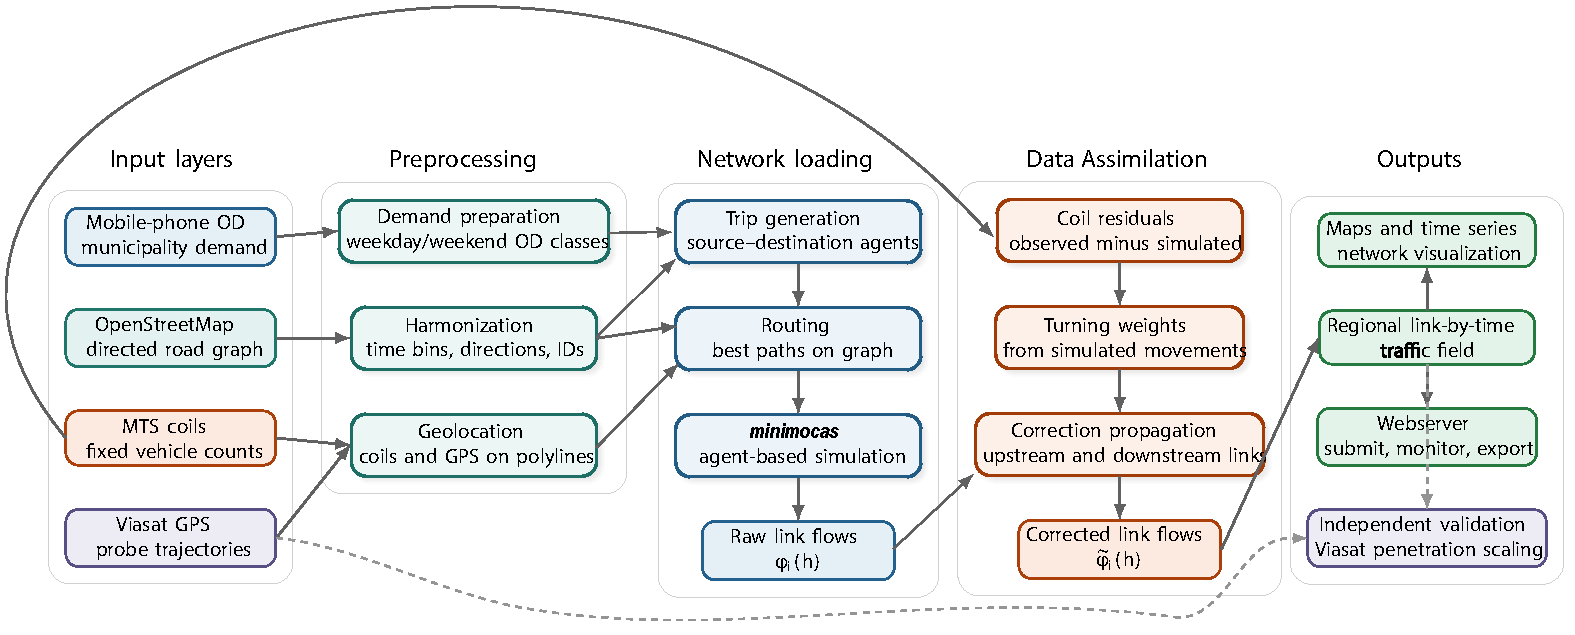
\includegraphics[width=.85\textwidth, height=0.70\textheight, keepaspectratio]{model_scheme.pdf}
  \caption{\textbf{End-to-end reconstruction workflow.}
  Mobile-phone OD activity defines regional demand, OpenStreetMap provides the directed road graph, MTS coils are geolocated on road polylines and Viasat
  GPS traces are kept for independent validation of the simulation framework. Demand is injected into the \texttt{minimocas} agent-based simulator, producing raw link flows. Coil
  residuals are then used for local data assimilation of the simulated counts and propagated through adjacent directed links using simulated turning
  weights. The final product is a data-assimilated link-by-time traffic field that can be mapped, validated against held-out GPS traces and exposed through the webserver.}
  \label{fig:workflow}
\end{figure}

\noindent Figure~\ref{fig:workflow} summarizes the logic of the reconstruction before the individual empirical results are presented. The workflow is
intentionally modular: mobile-phone data define demand, the road graph defines admissible movement, coils constrain local volumes through data assimilation, and GPS traces are held out for independent validation of the simulation framework. This separation makes the data-assimilation step interpretable because the information added by fixed counters is propagated through simulated turning structure rather than through a spatial smoothing rule unrelated to traffic direction.

\subsection{Observation layers and mobile-phone demand}

The reconstruction is carried out on the Emilia-Romagna regional road network, whose main structure is an east--west corridor connected to dense urban areas, coastal roads and Apennine links (Fig.~\ref{fig:inputs}a). The mobile-phone layer is aggregated at municipality level and converted into OD activity. Weekday activity in January 2020 is strongly concentrated along the regional urban corridor, especially around Bologna and the main provincial centres (Fig.~\ref{fig:inputs}b). This spatial heterogeneity is the demand signal that the model must redistribute onto individual road segments, following the general idea that aggregate mobility observations must be coupled to an explicit spatial network before they can inform link-level transport questions \cite{calabrese2011,toole2015,sheffi1985}.

The regional road traffic flow monitoring system (MTS) coils provide local vehicle counts on selected roads (Fig.~\ref{fig:inputs}c). Coil 282 is used as an illustrative fixed counter because it has a complete directional time series for the selected day and an unambiguous geographical record. Its 15-min profile displays the expected daily structure of a road counter: low night traffic, a morning increase and sustained afternoon activity (Fig.~\ref{fig:inputs}d). This combination of sparse fixed detectors and broader but sampled mobile traces is typical of traffic-state reconstruction problems
\cite{herrera2010,seo2017}.

\begin{figure*}[htbp]
  \centering
  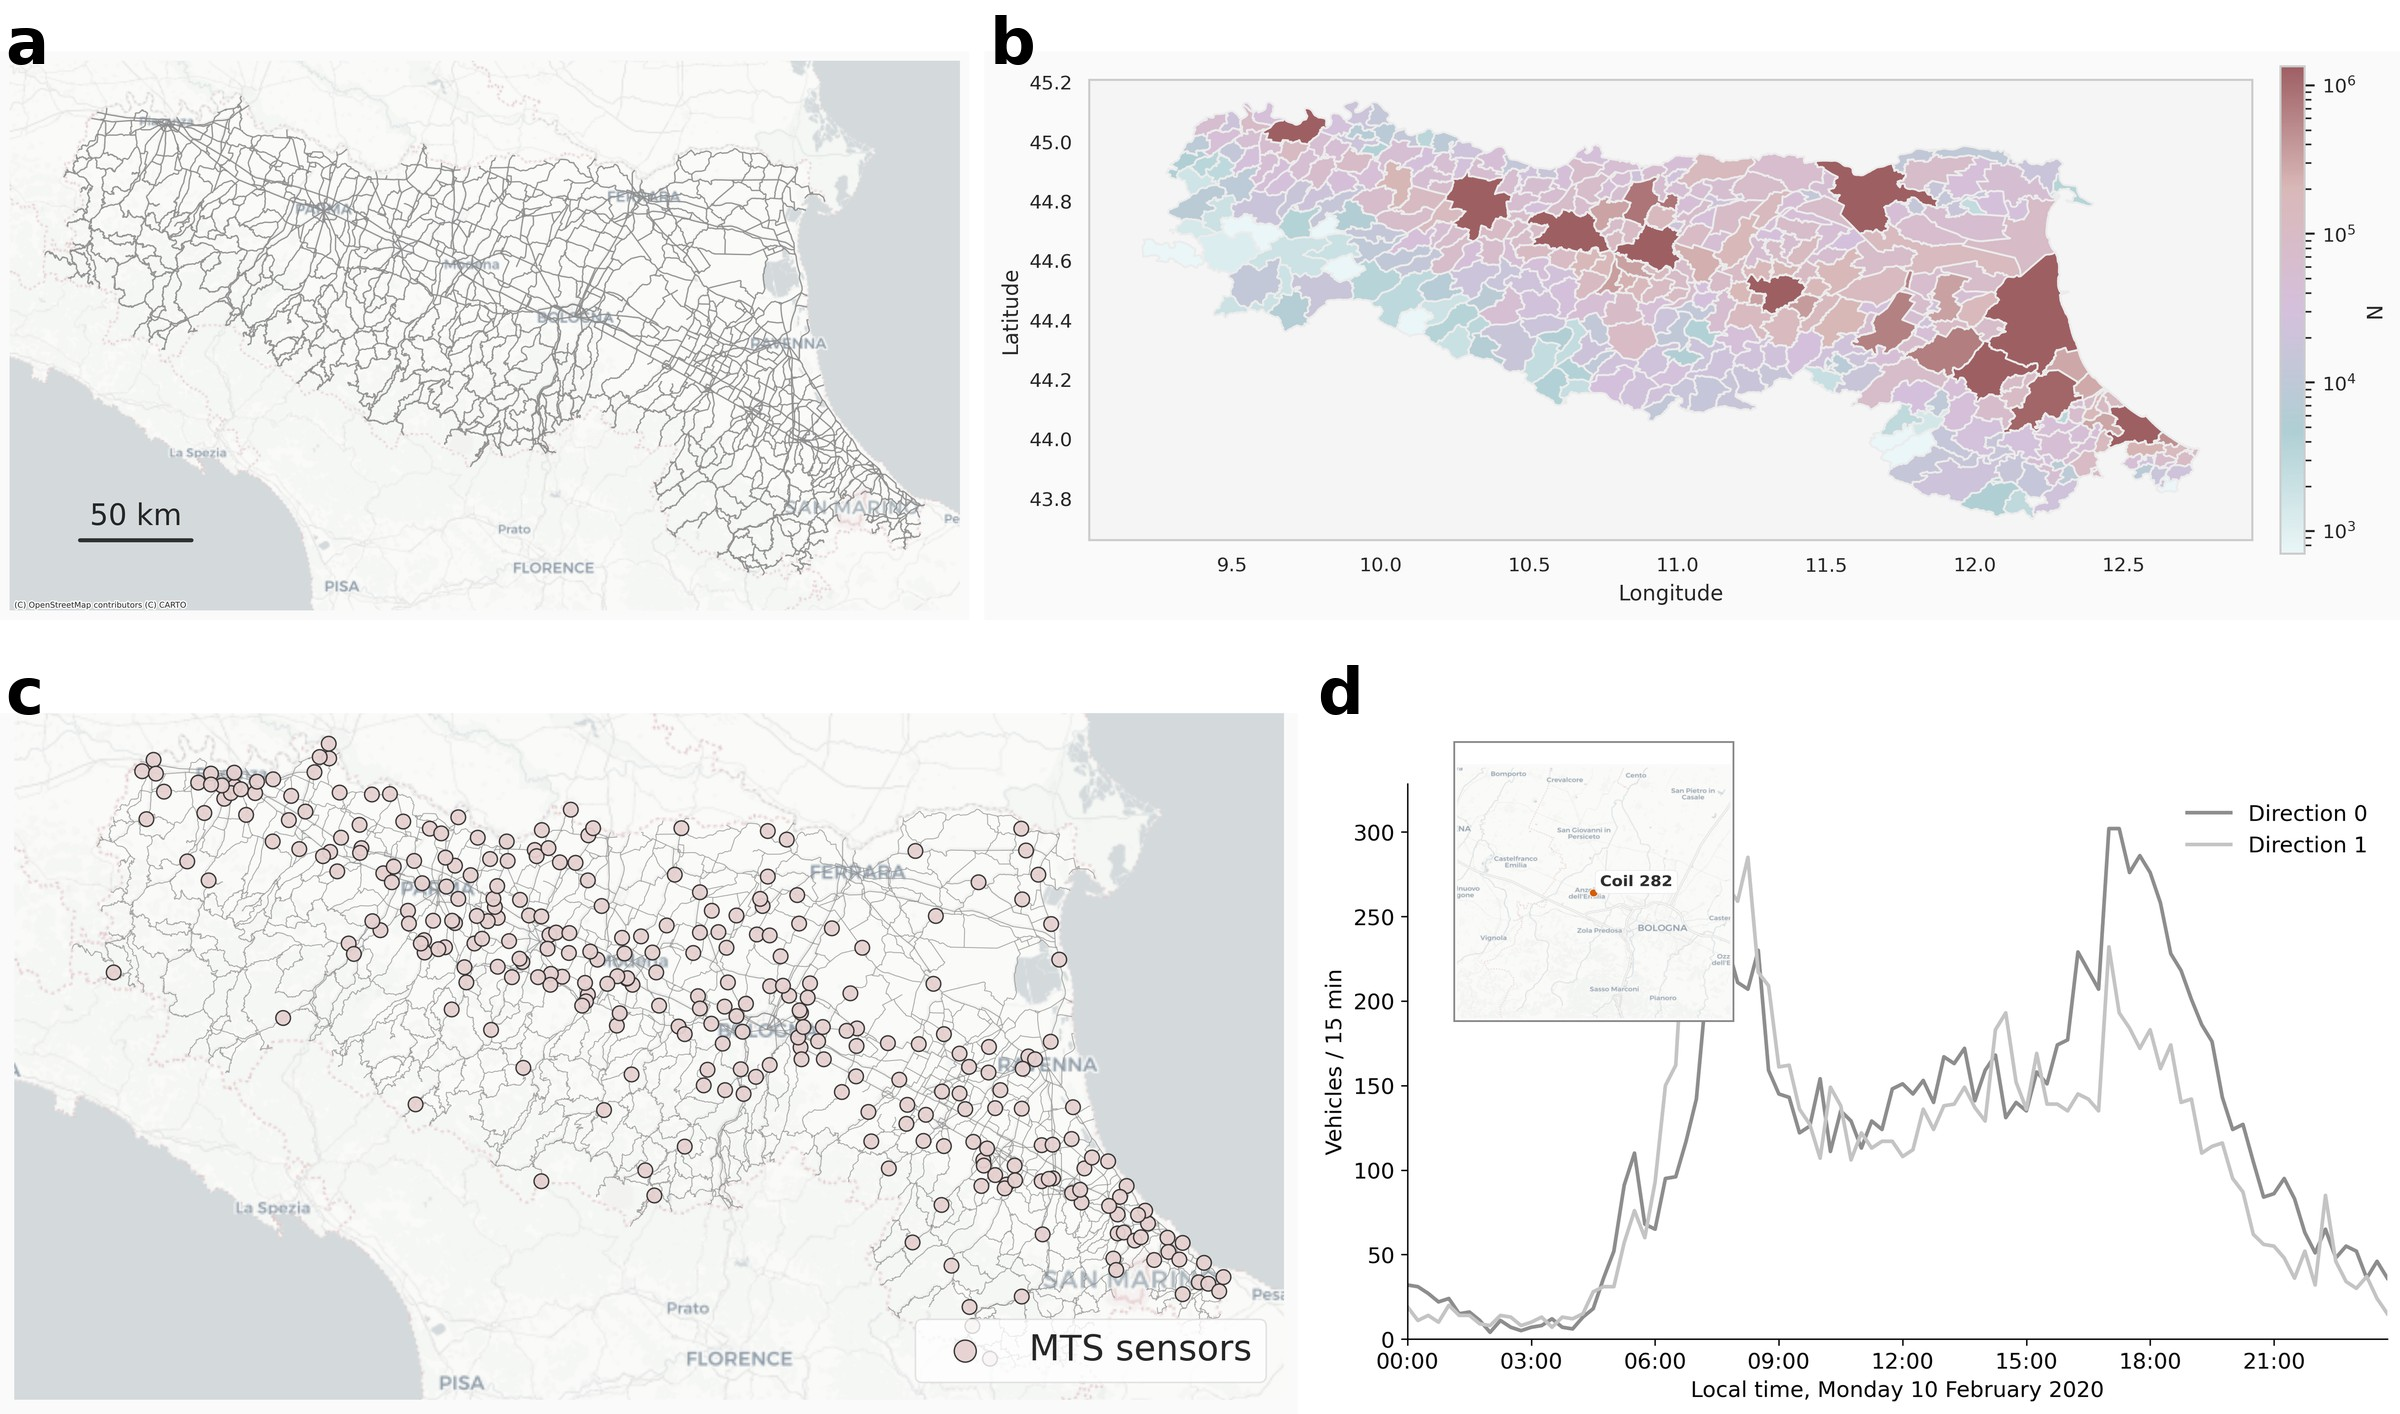
\includegraphics[width=\textwidth,height=.72\textheight,keepaspectratio]{fig1.jpg}
  \caption{\textbf{Study domain and observational inputs.}
  \textbf{(a)} Regional road cartography used by the model on a CartoDB
  Positron basemap; the scale bar corresponds to 50~km.
  \textbf{(b)} Weekday mobile-phone OD activity over Emilia-Romagna
  municipalities in January 2020; colour encodes activity $N$ on a
  logarithmic scale.
  \textbf{(c)} Locations of the MTS inductive loop detectors (coils) over the regional
  road graph.
  \textbf{(d)} Location of coil 282 (inset) and complete 15-min
  directional vehicle counts on Monday 10 February 2020, local time.}
  \label{fig:inputs}
\end{figure*}

The demand layer also contains temporal and categorical information. Mean weekday activity has a sharper morning peak and a stronger late-afternoon component than weekend activity (Fig.~\ref{fig:demand}a). The trip-generation classes indicate whether both endpoints are observed in the OD data or whether one or both endpoints are sampled from the modelled area (see Methods, Section~\ref{sec:data_preprocessing}).
Figure~\ref{fig:demand}b,c shows the mobility components used to decompose agent behaviour from the OD data. In both weekdays and weekends, the source--destination component dominates the reconstructed demand, while random-endpoint components represent residual mobility that cannot be directly linked to two observed municipalities. These classes are not arbitrary noise: they regularize weakly observed OD mass, prevent sparse low-count pairs from generating deterministic routes with false precision, preserve regional coverage and avoid an artificial collapse of weakly observed mobility onto a small number of high-count municipality pairs. Ranking municipalities by activity confirms that a small number of urban centres drive a large fraction of the demand (Fig.~\ref{fig:demand}d), consistent with empirical evidence that human mobility is highly heterogeneous across places and distances \cite{gonzalez2008,simini2012,lenormand2016}.

\begin{figure*}[htbp]
  \centering
  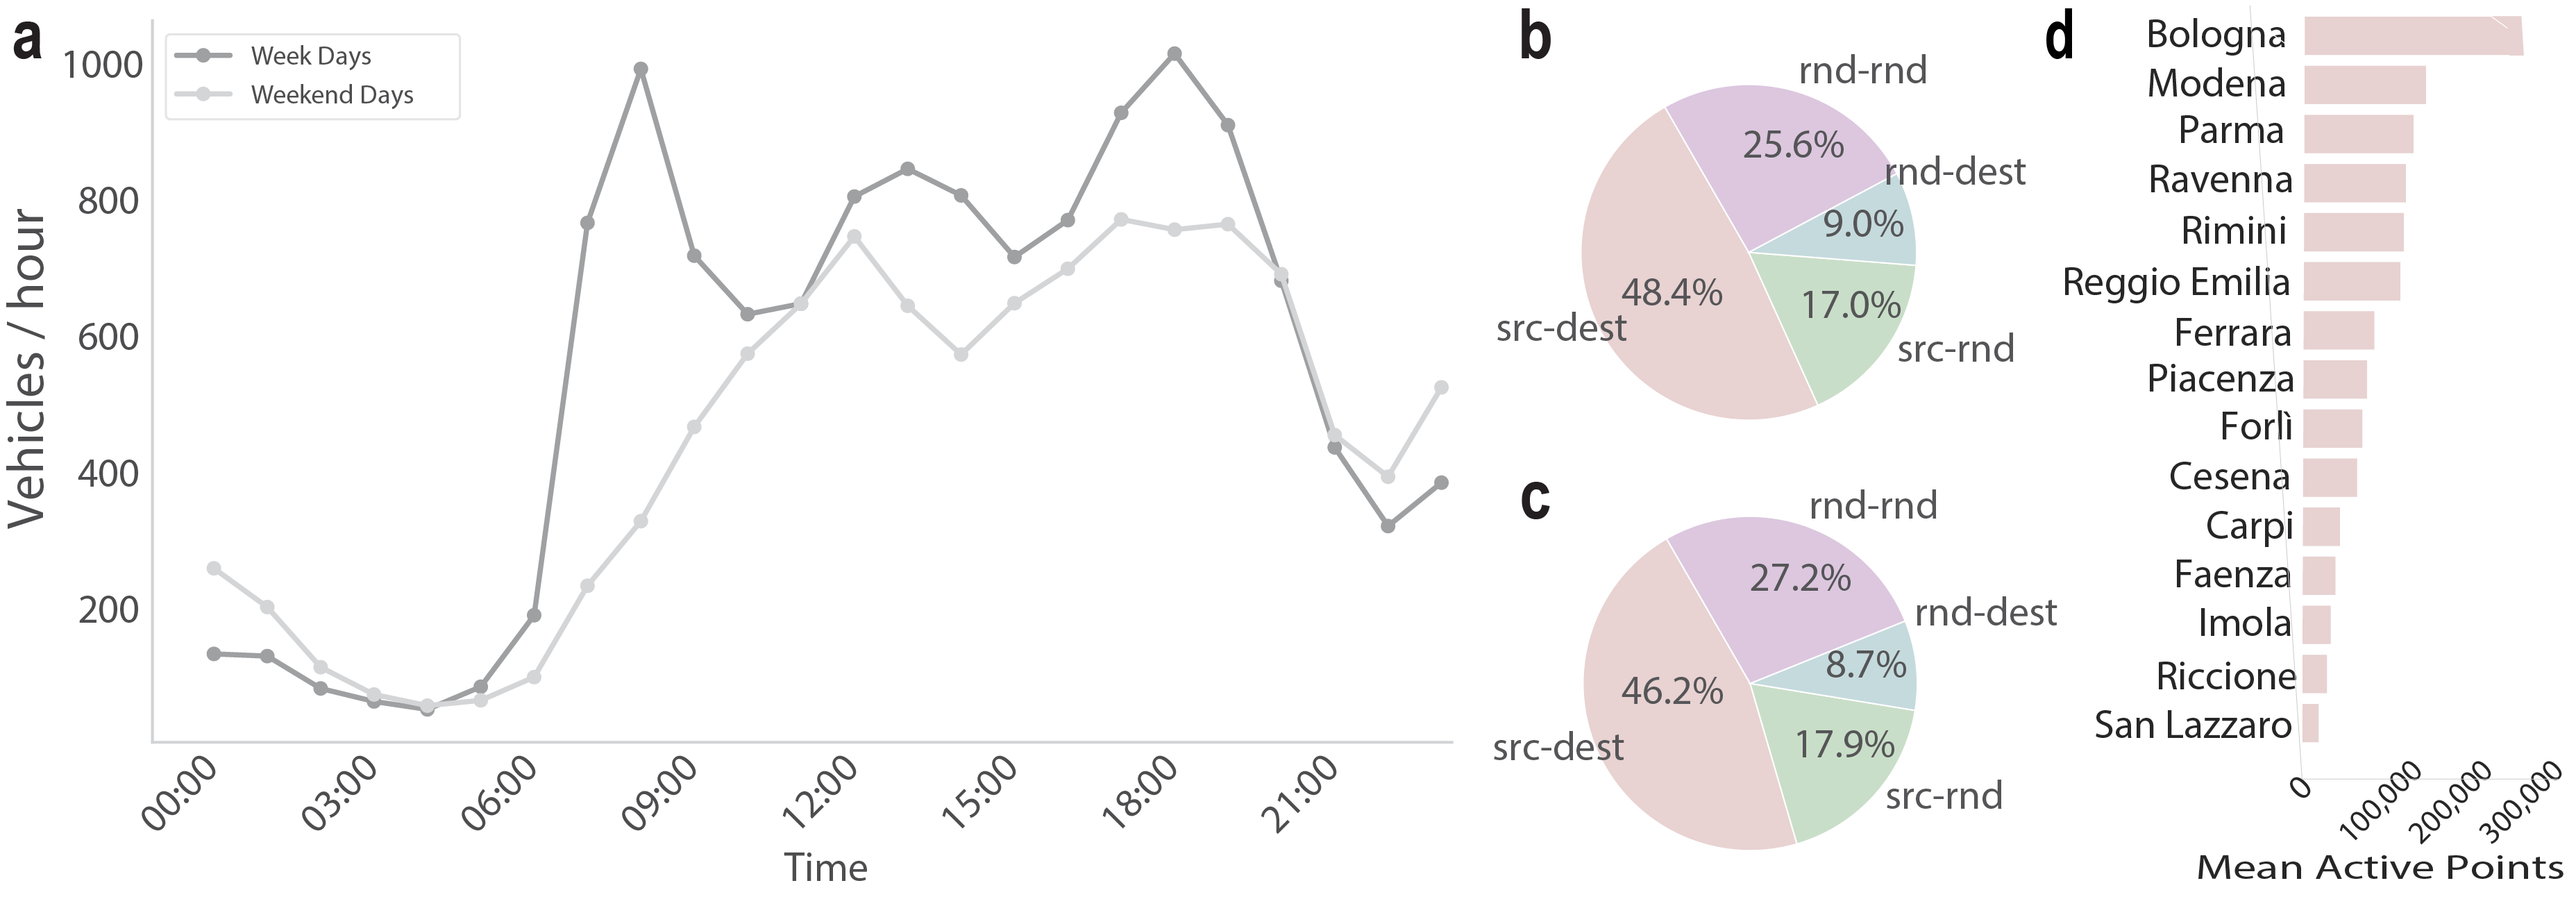
\includegraphics[width=\textwidth,height=.72\textheight,keepaspectratio]{fig2.png}
  \caption{\textbf{Mobile-phone demand used to drive the reconstruction.}
  \textbf{(a)} Mean hourly OD activity profiles for weekdays and weekend
  days in January 2020.
  \textbf{(b)} Weekday and \textbf{(c)} weekend shares of the four
  generation classes: source--destination (\texttt{src-dest}),
  source--random (\texttt{src-rnd}), random--destination
  (\texttt{rnd-dest}) and random--random (\texttt{rnd-rnd}).
  \textbf{(d)} Ranking of the most active municipalities by mean mobile
  activity; the plot reports the first 10 and last 10 municipalities among
  the top 50.}
  \label{fig:demand}
\end{figure*}

\subsection{Network reconstruction and local counter control}

The simulation converts the OD demand into directional link flows. For each hour, generated agents are placed on the directed road graph, routed toward their destination and counted on every traversed polyline. The output is a link-by-time matrix $\phi_i(h)$, where $i$ is a road polyline and $h$ is the hour. The comparison with coil 282 shows that the simulated road associated with the counter follows the same broad daily structure as the observed series on Monday 10 February 2020, a working day before the COVID-19 mobility restrictions (Fig.~\ref{fig:simulation}a). The map of simulated daily flows highlights the high-volume regional corridors while retaining non-zero information on the secondary network (Fig.~\ref{fig:simulation}b). This microscopic-to-link aggregation follows the logic of agent-based traffic simulators, where individual vehicle trajectories are used to recover network-level flow fields
\cite{horni2016,lopez2018,treiber2013}.

\begin{figure*}[htbp]
  \centering
  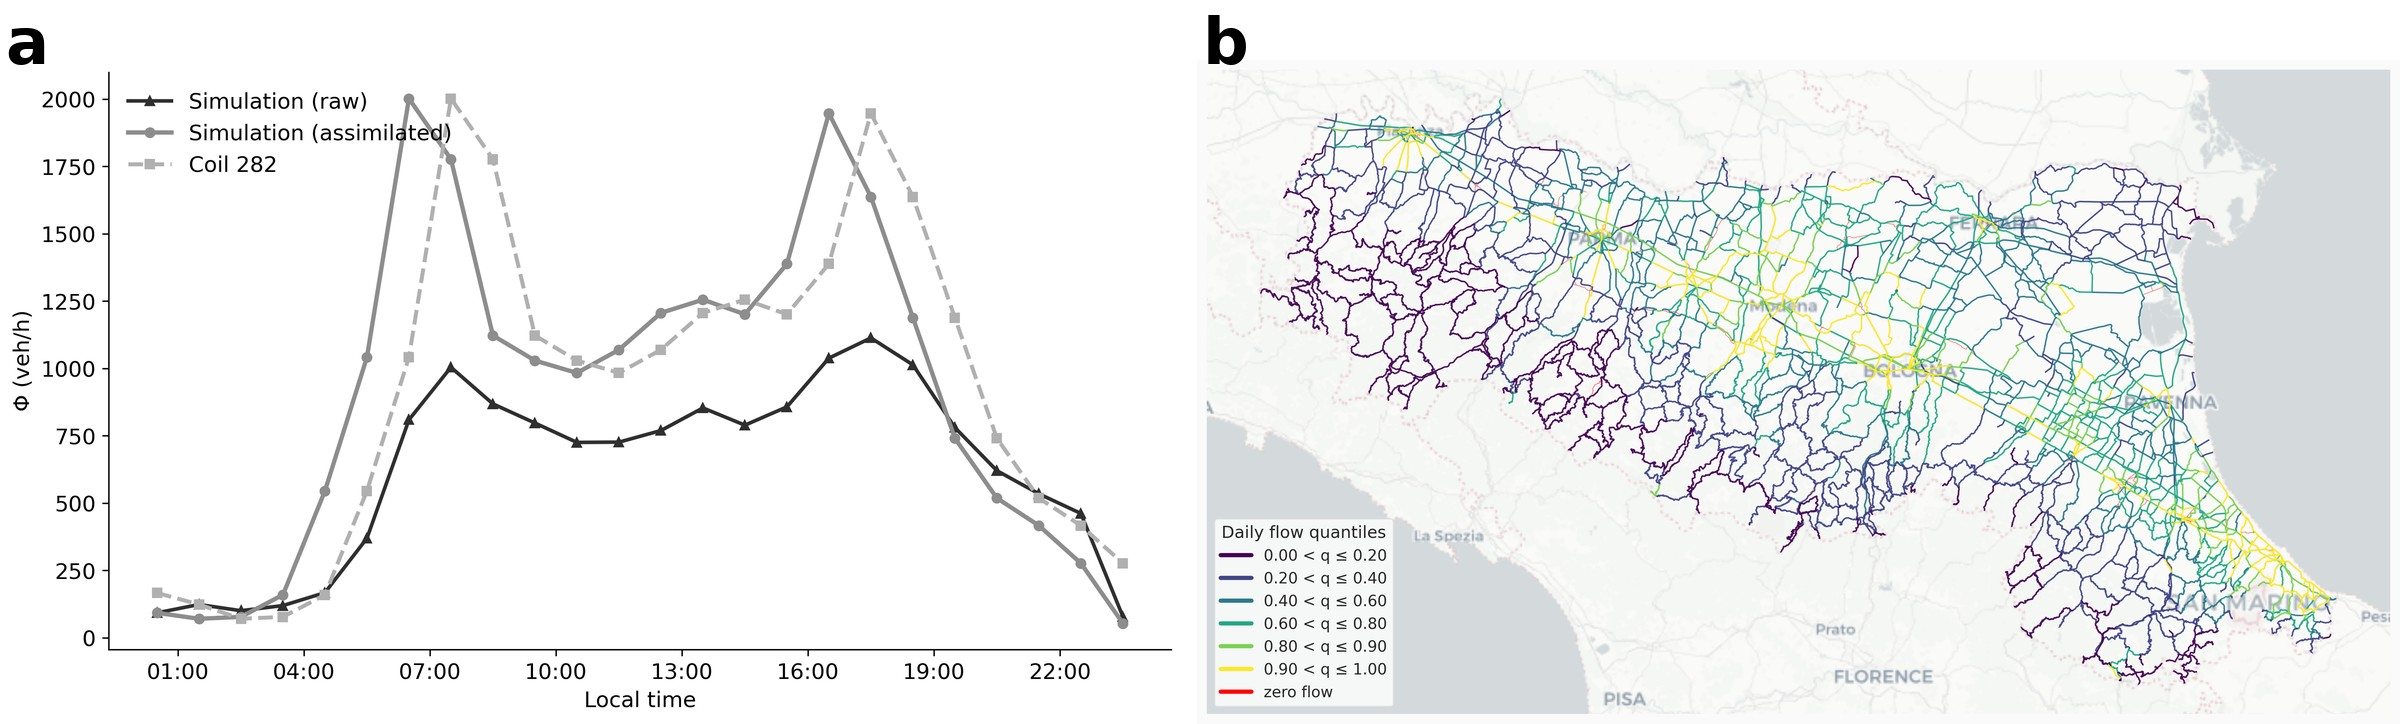
\includegraphics[width=\textwidth,height=.72\textheight,keepaspectratio]{fig3.jpg}
  \caption{\textbf{Link-level reconstruction output.}
  \textbf{(a)} Hourly simulated flow on the polyline associated with coil
  282 compared with hourly aggregated coil observations on Monday
  10 February 2020; $\Phi$ denotes vehicle flow.
  \textbf{(b)} Spatial distribution of simulated daily link flows over
  Emilia-Romagna, expressed through flow quantile classes; yellow segments
  carry the highest reconstructed flows and purple segments the lowest.}
  \label{fig:simulation}
\end{figure*}

\subsection{Accident exposure}

The reconstructed field can serve as an exposure denominator for aggregate accident statistics. The regional accident tables for 2022--2024 (16,679, 16,808 and 16,757 accidents) give counts by hour of the day and by road type, with no location. Let $A(h)$ be the share of accidents in hour $h$ and $E(h)$ the share of simulated vehicles on the whole network in the same hour (Fig.~\ref{fig:temporal_risk}a). We define the relative risk
\begin{equation}
  R(h) = \frac{A(h)/E(h)}{\frac{1}{24}\sum_{h'} A(h')/E(h')} ,
  \label{eq:hourly_risk}
\end{equation}
which equals one on average over the day. With weekday exposure, $R$ is 3.4 at 00:00 and 2.4 at 01:00, stays between 1.0 and 1.4 from 03:00 to 07:00, and is below 0.6 after 19:00 (Fig.~\ref{fig:temporal_risk}b). The night values rest on the simulated night exposure, the least reliable part of the simulated profile (Section~\ref{sec:limitations}). Ward clustering of the hourly risk and exposure values separates three regimes: night (21:00--06:00), morning (07:00--09:00) and day (10:00--20:00) (Fig.~\ref{fig:temporal_risk}c).

A least-squares fit of $\log A$ against $\log E$ on the 24 hourly points gives $A \sim E^\alpha$ with $\alpha = 0.72$, 95\% bootstrap confidence interval 0.58--0.88 (10,000 resamples of the 24 hours), and $R^2 = 0.85$ (Fig.~\ref{fig:temporal_risk}d). Across hours, the accident share grows less than proportionally with the simulated exposure.

\begin{figure*}[htbp]
  \centering
  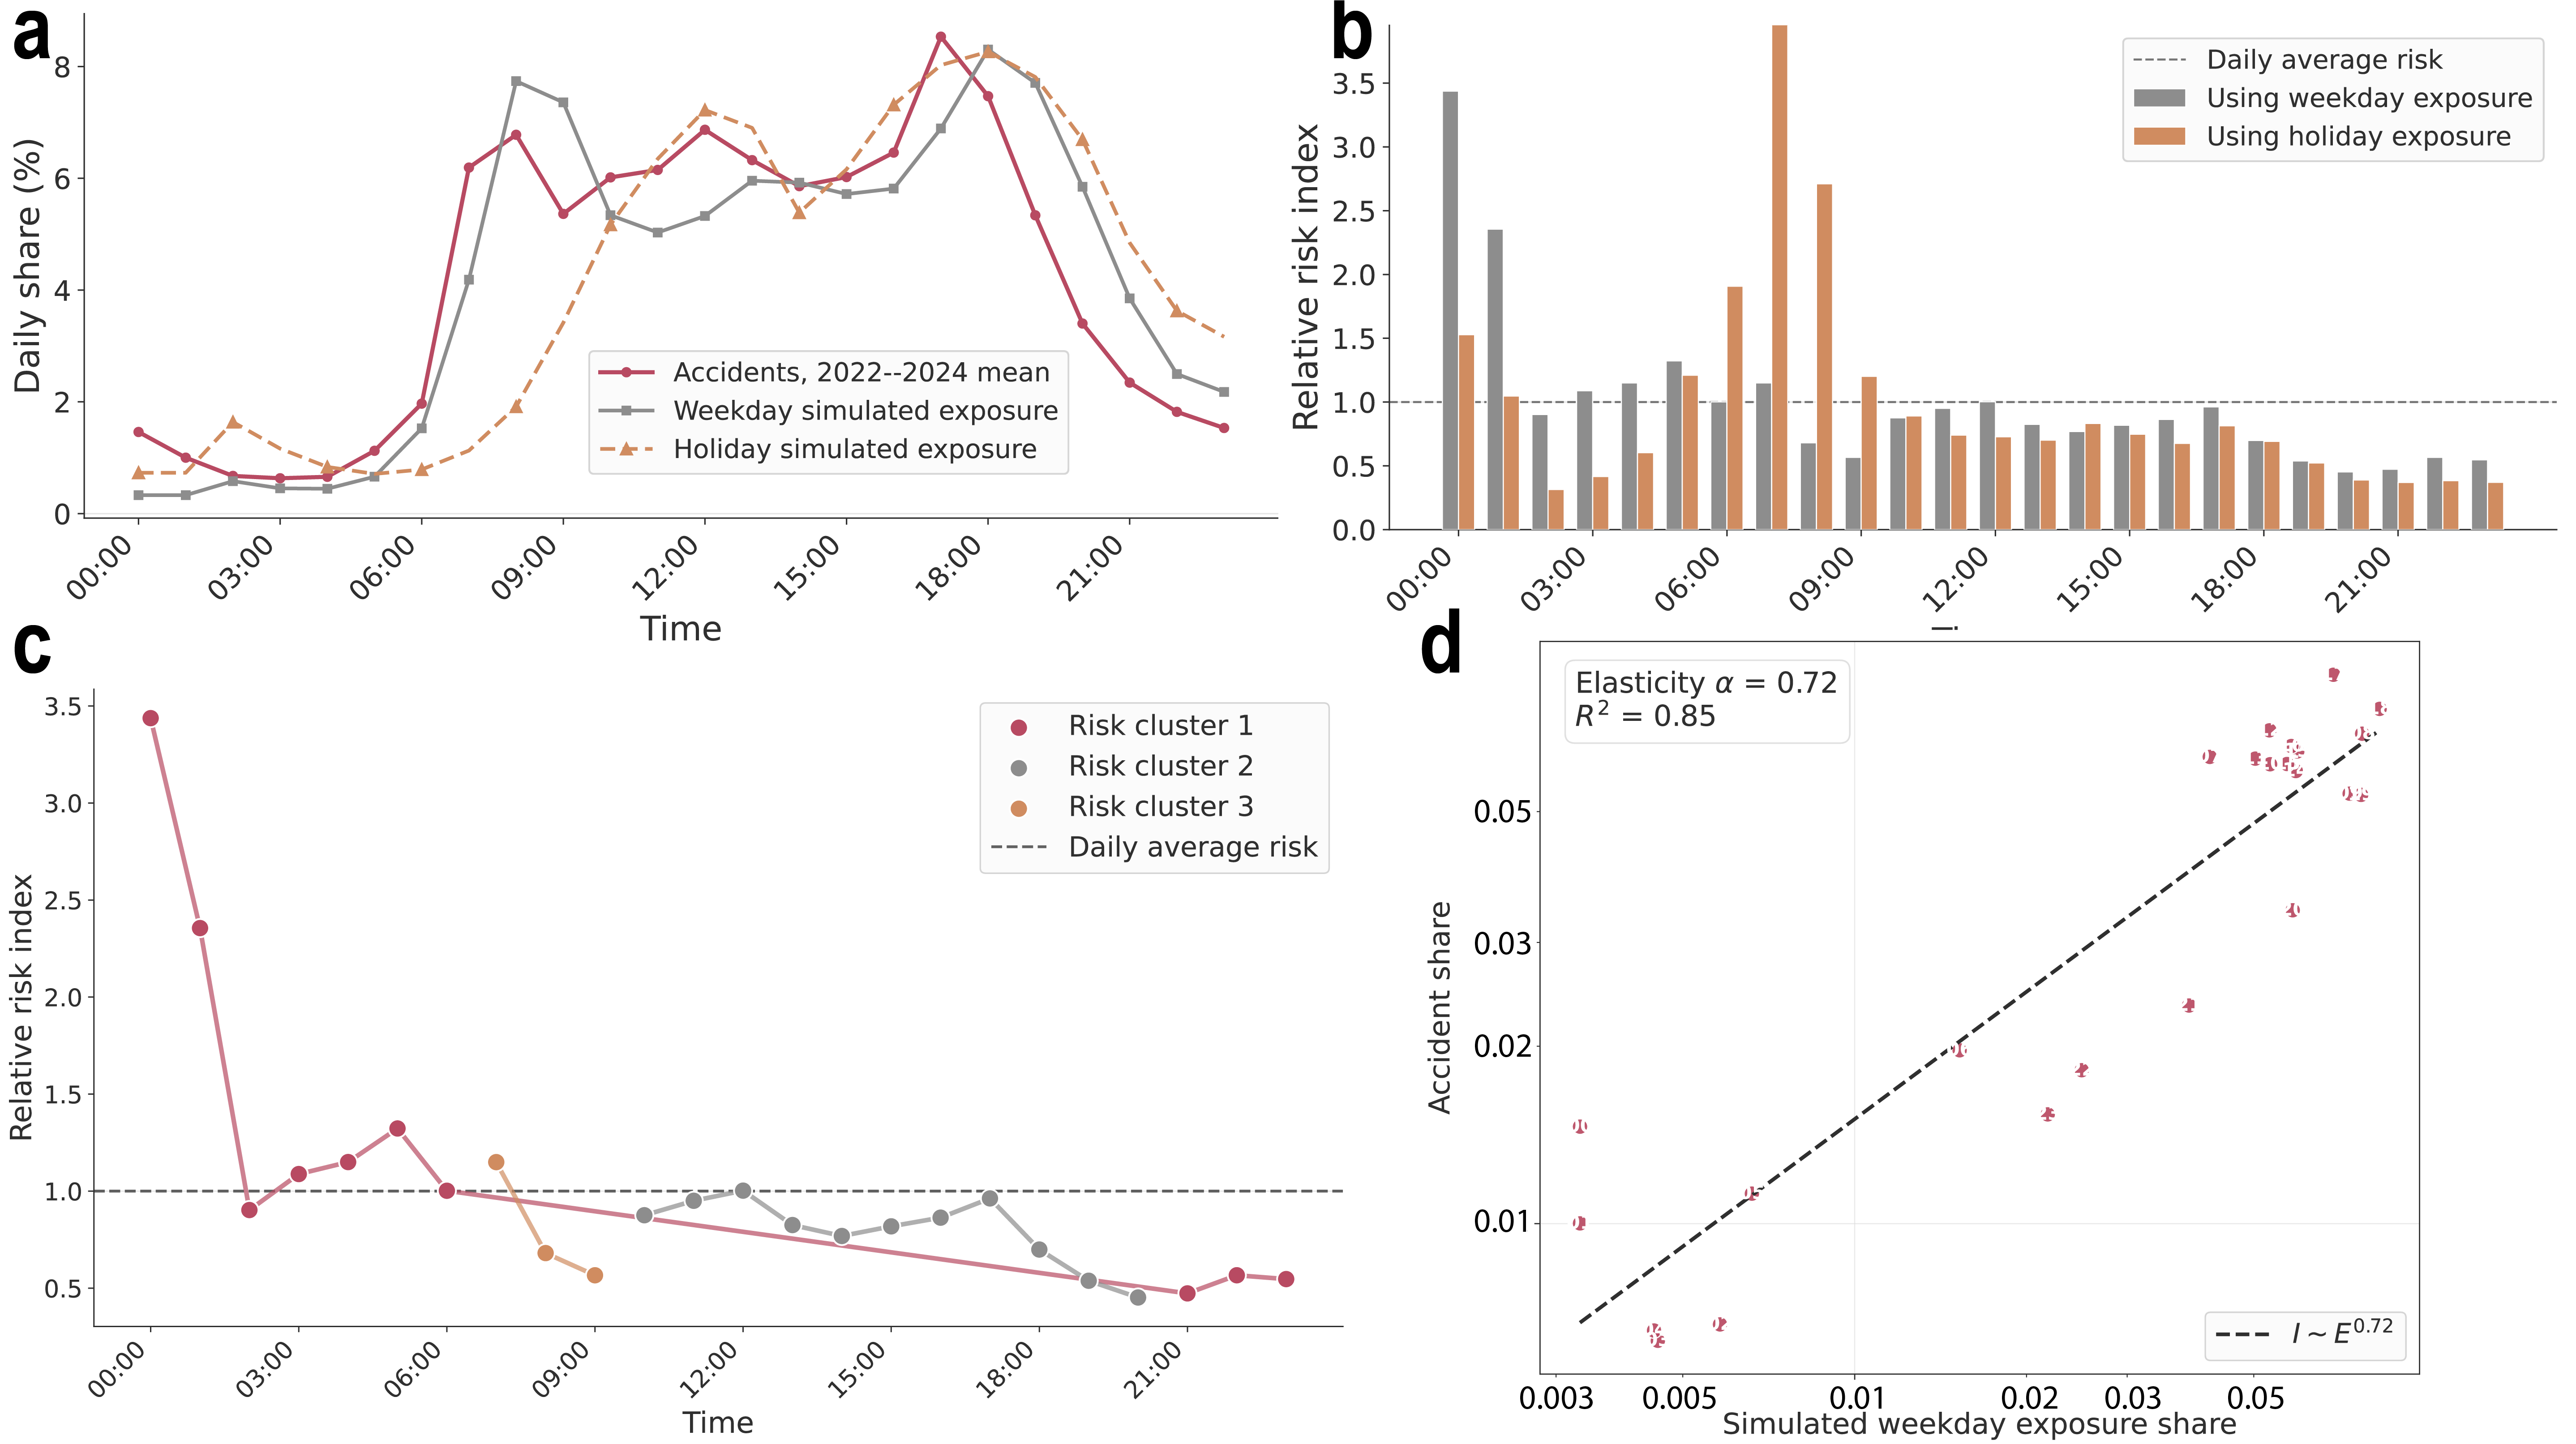
\includegraphics[width=\textwidth,height=.72\textheight,keepaspectratio]{fig7.png}
  \caption{\textbf{Accidents and simulated exposure by hour.}
  \textbf{(a)} Hourly accident share (mean of 2022--2024) and simulated weekday and weekend exposure shares.
  \textbf{(b)} Relative risk $R(h)$, Eq.~\eqref{eq:hourly_risk}, with weekday (grey) and weekend (orange) exposure; the dashed line marks $R=1$.
  \textbf{(c)} Three hourly regimes from Ward clustering of risk and exposure values.
  \textbf{(d)} Accident share against simulated weekday exposure share for the 24 hours (log--log axes) and fit $A\sim E^{\alpha}$, $\alpha = 0.72$ (95\% bootstrap interval 0.58--0.88), $R^2 = 0.85$.}
  \label{fig:temporal_risk}
\end{figure*}

$R(h)$ is a regional profile and is the same for every link. The hazard-weighted exposure $H_i$ of a link (Eq.~\eqref{eq:hazard_weighted_exposure}, Fig.~\ref{fig:spatial_risk}a) is therefore its simulated volume weighted by the hourly composition of its traffic, and the rank difference $S_i$ (Eq.~\eqref{eq:hazard_anomaly}, Fig.~\ref{fig:spatial_risk}e) picks out links that carry a larger share of their traffic in high-$R$ hours. The risk centrality $C_i$ (Fig.~\ref{fig:spatial_risk}c,d) and the weekday--weekend contrast $D_i$ (Fig.~\ref{fig:spatial_risk}b) follow the same logic. These maps show where simulated traffic coincides with hours of high regional risk; they carry no information on where accidents occur. Supplementary Fig.~S3 gives the yearly totals, road types and seasonal shares of the accident data.

\begin{figure*}[htbp]
  \centering
  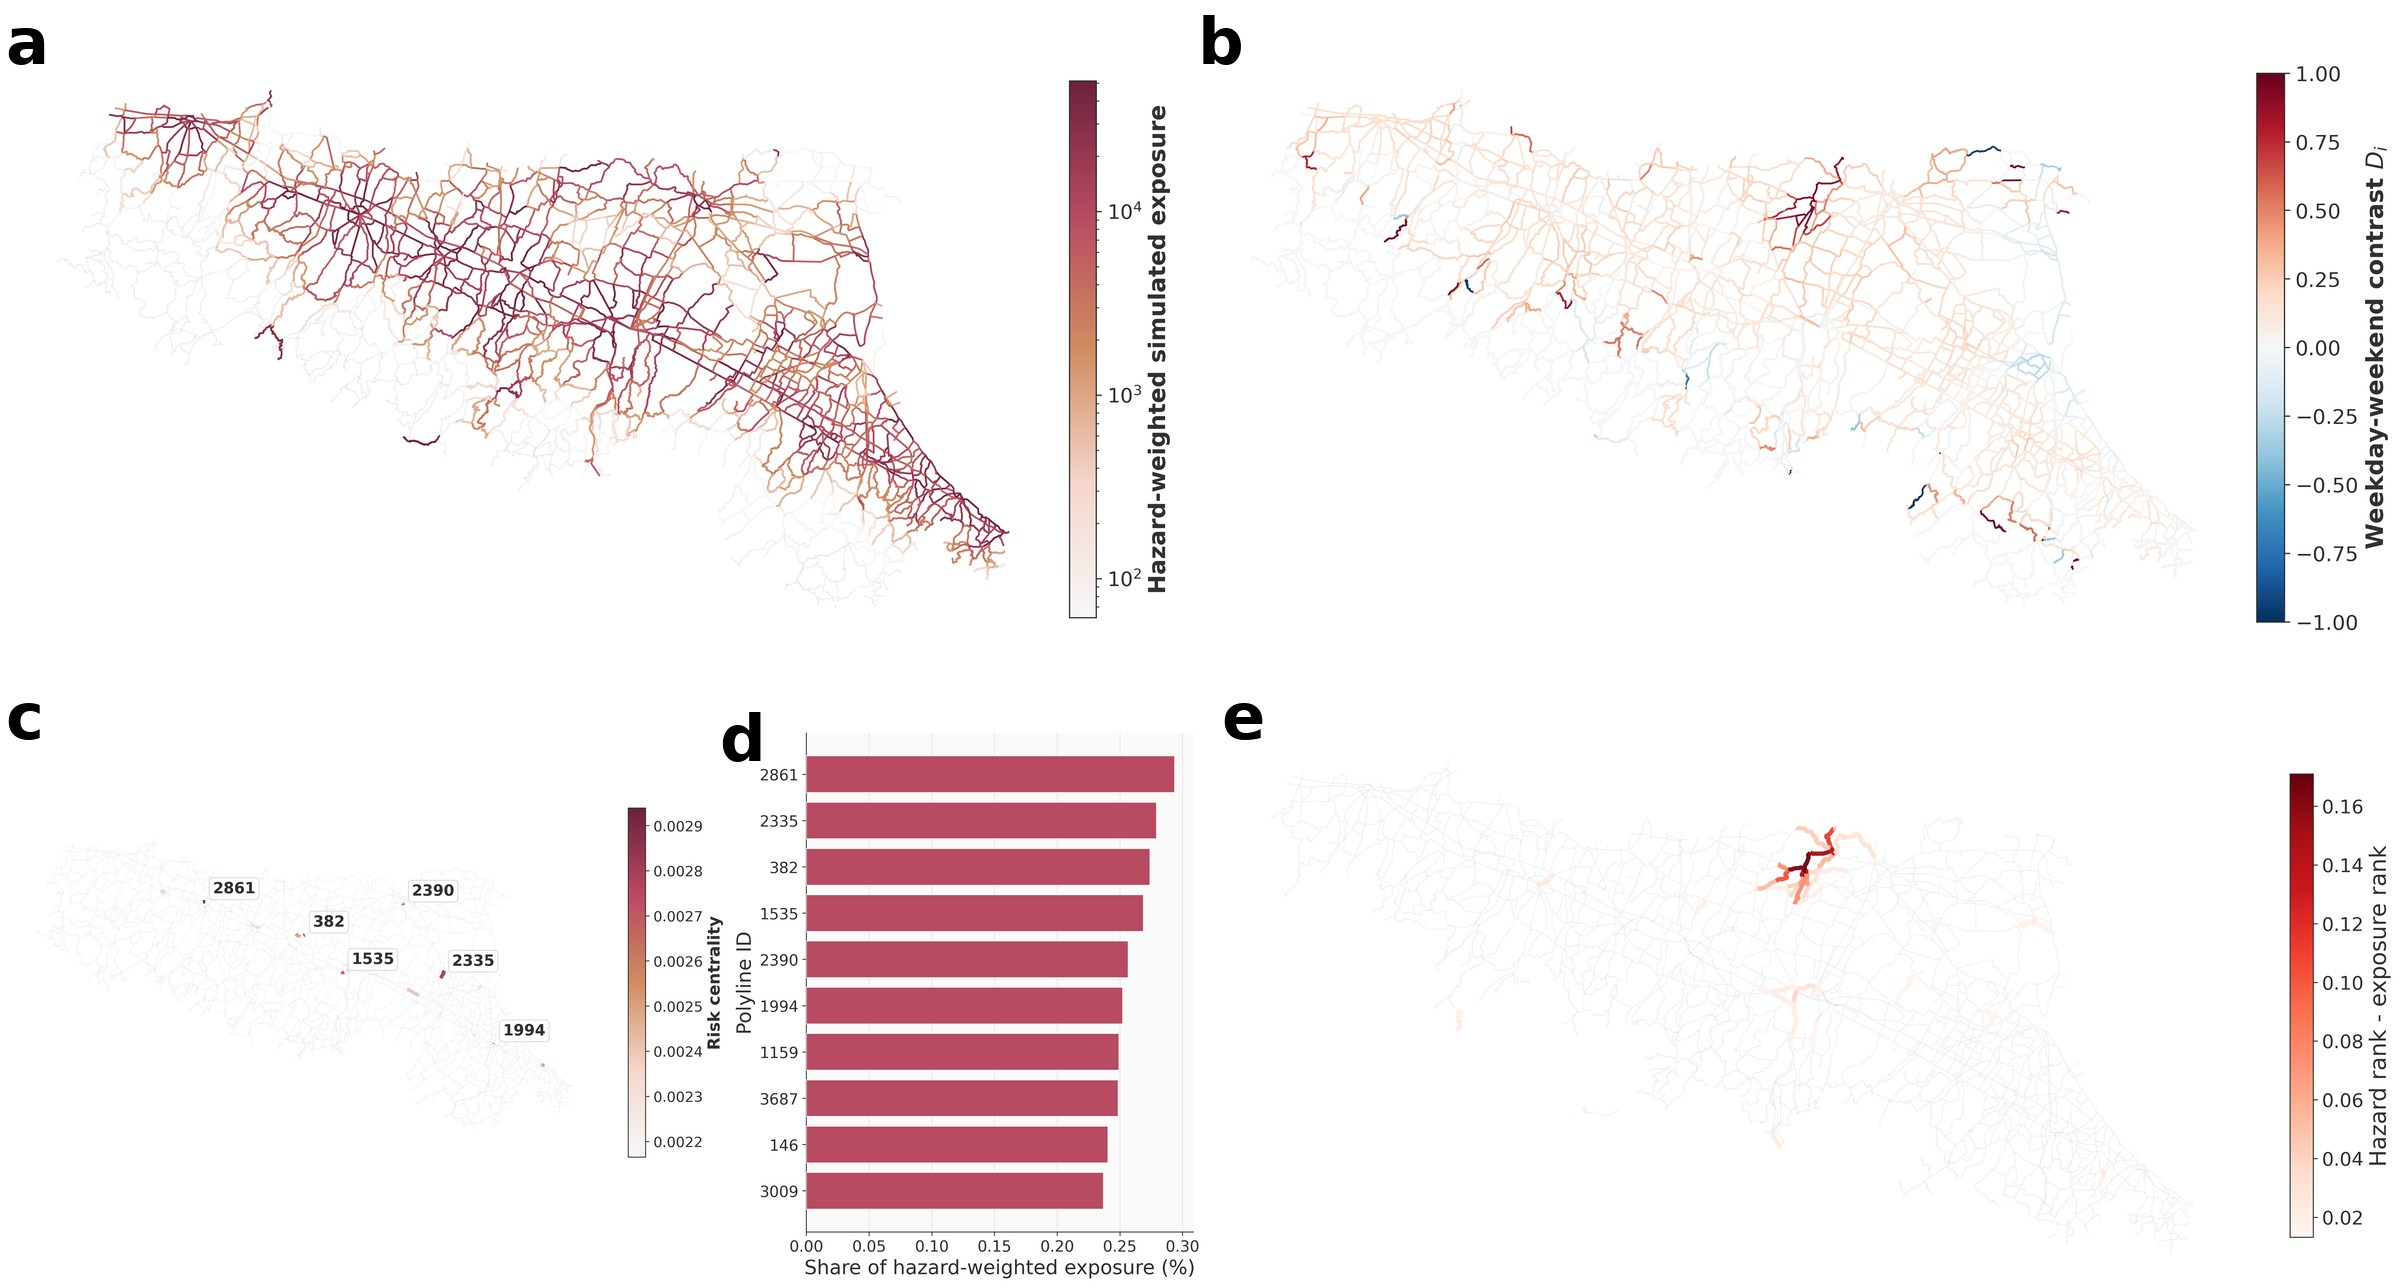
\includegraphics[width=\textwidth,height=.72\textheight,keepaspectratio]{fig8.jpg}
  \caption{\textbf{Simulated weekday exposure weighted by the regional risk profile.}
  \textbf{(a)} Hazard-weighted exposure $H_i$, Eq.~\eqref{eq:hazard_weighted_exposure}.
  \textbf{(b)} Weekday--weekend contrast $D_i$, Eq.~\eqref{eq:weekday_weekend_hazard_difference}; positive values mark links with larger weekday $H_i$.
  \textbf{(c)} Location of the links with the highest risk centrality $C_i$, Eq.~\eqref{eq:risk_centrality}, and \textbf{(d)} their share of the total hazard-weighted exposure.
  \textbf{(e)} Links in the top 5\% of the rank difference $S_i$, Eq.~\eqref{eq:hazard_anomaly}.}
  \label{fig:spatial_risk}
\end{figure*}

\subsection{Independent Viasat validation}

Viasat GPS observations give an independent test of the hourly profiles produced by the reconstruction; they enter neither the demand nor the assimilation. Matched Viasat links cover only part of the regional cartography, mostly in the Forl\`i--Cesena area (Fig.~\ref{fig:viasat}a,d). For each matched polyline $i$ we estimate the penetration coefficient
\begin{equation}
  \eta_i =
  \frac{\sum_{d}\sum_h \psi_i(d,h)}{\sum_{d}\sum_h \phi_i(d,h)},
  \label{eq:penetration}
\end{equation}
where $\psi_i(d,h)$ is the number of Viasat probes on day $d$ and hour $h$, $\phi_i(d,h)$ is the simulated flow, and both sums run over the same days of the validation interval. The penetration-normalized GPS profile is
\begin{equation}
  \widetilde{\psi}_i(h) = \frac{1}{\eta_i}\sum_d \psi_i(d,h) .
  \label{eq:normalized_gps}
\end{equation}
The rescaling sets the GPS volume of each road equal to the simulated one and leaves the hourly shape unchanged, so the comparison tests when traffic occurs on each link and says nothing about the size of the Viasat fleet. A link-specific factor is needed because probe coverage varies strongly across the network \cite{herrera2010,seo2015,seo2017}.

Validation compares the hourly shares $p_i(h)=\phi_i(h)/\sum_{h'}\phi_i(h')$ and $q_i(h)=\widetilde{\psi}_i(h)/\sum_{h'}\widetilde{\psi}_i(h')$, where $\phi_i(h)=\sum_d\phi_i(d,h)$; the shares do not depend on $\eta_i$. The profile error of link $i$ is the mean absolute error over the 24 hours, in percentage points (pp),
\begin{equation}
  \mathrm{MAE}_i = \frac{100}{24}\sum_{h=0}^{23}
  \bigl| p_i(h) - q_i(h) \bigr| ,
  \label{eq:profile_error}
\end{equation}
and we also report it relative to the mean hourly share $100/24 \simeq 4.17$~pp,
\begin{equation}
  \varepsilon_i = \frac{\mathrm{MAE}_i}{100/24} = \sum_{h=0}^{23} \bigl| p_i(h) - q_i(h) \bigr| ,
  \label{eq:relative_error}
\end{equation}
which is the $L^1$ distance between the two daily distributions: $\varepsilon_i=0$ for identical profiles and $\varepsilon_i=2$ for profiles with disjoint support.

The penetration spans four decades (Fig.~\ref{fig:viasat}b,e). In 2020 the median $\eta_i$ is 0.50\%; the classes $\eta\sim10^{-2}$ and $\eta\sim10^{-3}$ contain 60.6\% and 32.4\% of the 848 usable links, and only 17 links (2.0\%) reach $\eta\sim10^{-1}$. In 2021 the median is 0.44\% and the two main classes contain 61.3\% and 34.2\% of 845 links. The classes are interwoven in space (Fig.~\ref{fig:viasat}c,f): penetration is a property of individual roads more than of an area.

\begin{figure*}[htbp]
  \centering
  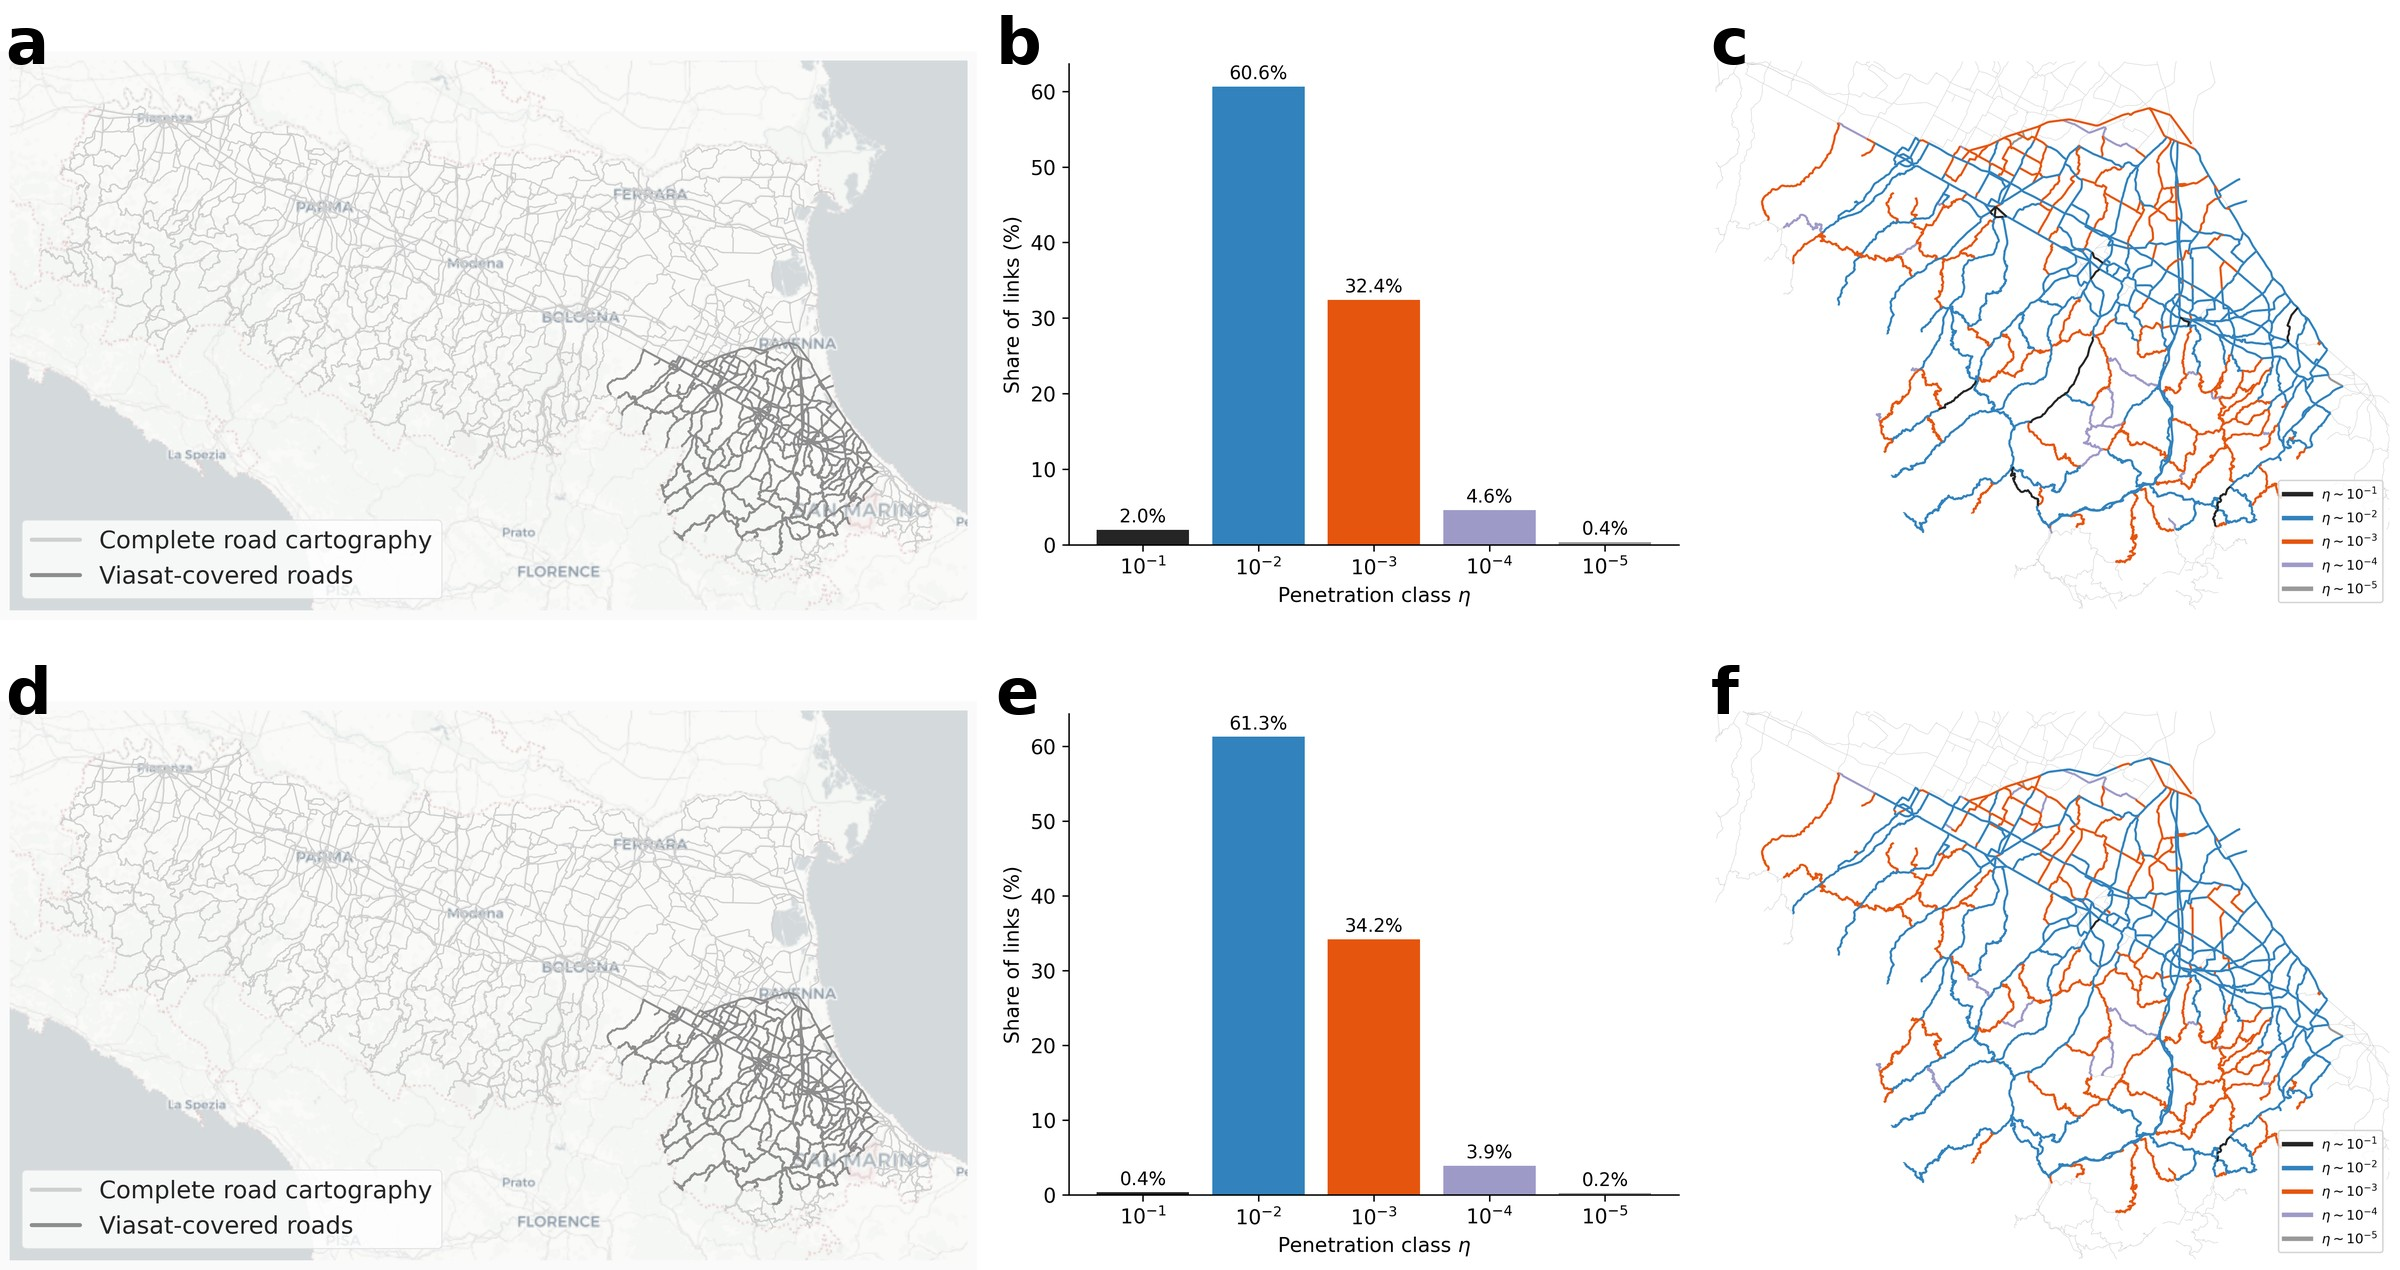
\includegraphics[width=\textwidth,height=.72\textheight,keepaspectratio]{fig4.jpg}
  \caption{\textbf{Viasat coverage and link penetration.}
  Top row: validation interval 10--17 February 2020.
  Bottom row: validation interval 28 June--4 July 2021.
  \textbf{(a,d)} Matched Viasat links (dark grey) over the complete regional
  road graph (light grey).
  \textbf{(b,e)} Share of usable links in each penetration class, $\eta_i$ rounded to the nearest power of ten.
  \textbf{(c,f)} Geographical distribution of the same classes
  in the Forl\`i--Cesena validation area.}
  \label{fig:viasat}
\end{figure*}

\subsection{Profile errors on all matched links}

We compute $\mathrm{MAE}_i$ on every matched link with non-zero simulated and GPS totals, 848 of the 930 matched links in 2020 and 845 of 927 in 2021. Simulation and GPS cover the same days: eight in 2020 (six weekdays and the weekend of 15--16 February) and seven in 2021 (five weekdays and the weekend of 3--4 July), with weekend days simulated from the weekend OD matrix. Table~\ref{tab:validation_all} and Fig.~\ref{fig:validation_cdf} summarize the distributions.

The median MAE is 1.34~pp in 2020 and 1.49~pp in 2021, i.e.\ a relative error $\varepsilon$ of 32\% and 36\% of the mean hourly share. The error depends strongly on penetration. On the 514 links with $\eta\sim10^{-2}$ the 2020 median is 1.13~pp ($\varepsilon=27\%$), on the 275 links with $\eta\sim10^{-3}$ it is 2.13~pp ($\varepsilon=51\%$), and on the 39 links with $\eta\sim10^{-4}$ the GPS profile is dominated by counting noise ($\varepsilon=123\%$). The 2021 values are similar (Table~\ref{tab:validation_all}).

Part of the error is a systematic lead of the simulation. Summed over all usable links, the simulated profile peaks at 17:00 and the Viasat profile at 18:00 in both campaigns, and the MAE of the two aggregate profiles is 0.69~pp (2020) and 0.82~pp (2021). Shifting the simulated profiles forward by one hour lowers the median link MAE to 1.29 and 1.34~pp. We do not apply this shift, since the simulator output and the Viasat tables both label each hour by its start; the possible origins of the lead are discussed in Section~\ref{sec:limitations}.

To judge these values we apply two fixed profiles to every link and compute the same error (Table~\ref{tab:baselines}). The first is the hourly profile of the OD demand injected in the runs, summed over the same days; it measures what the network loading adds to the timing of the demand. The second is the mean normalized hourly profile of the MTS coils: the 82 coil directions with complete data on all eight days in 2020 and, since no observed coil table covers June--July 2021, the summer weekday averages of 471 coil directions from the 2022 archive. The reconstruction has a lower error than the OD profile on 74\% of the links in 2020 and 76\% in 2021, but the gain is small, from 1.40 to 1.34~pp and from 1.52 to 1.49~pp in median. The MTS mean profile does better than the reconstruction: its median MAE is 1.15~pp in 2020 and 1.21~pp in 2021, and its error is lower on 91\% and 87\% of the links. On the $\eta\sim10^{-2}$ class of 2020 the medians are 0.82~pp for the MTS profile and 1.13~pp for the reconstruction. A generic counter profile therefore describes the timing of traffic on the Viasat links better than the simulation, which takes its timing from the OD demand and anticipates the observed peaks by about one hour. What the reconstruction adds is a volume for every directed link and its spatial distribution, which no single profile provides; its hourly shape on unobserved links is its weakest component.

\begin{table}[htbp]
\centering
\caption{Median and interquartile range of the link MAE (pp) for the reconstruction and for two profiles applied identically to every link: the hourly profile of the injected OD demand and the mean normalized profile of the MTS coils (2020: the 82 coil directions with complete data on all eight validation days; 2021: summer weekday averages of 471 coil directions from the 2022 MTS archive). The last column gives the percentage of links on which the assimilated simulation has a lower MAE than the baseline.}
\label{tab:baselines}
\begin{tabular}{@{}llrrr@{}}
\toprule
Campaign & Profile & Median MAE & IQR & Simulation better [\%] \\
\midrule
2020 & Simulation (assimilated) & 1.34 & 1.05--2.01 & -- \\
 & Simulation (raw) & 1.33 & 1.02--1.99 & -- \\
 & Simulation shifted by $+1$~h & 1.29 & 0.92--1.97 & -- \\
 & OD demand profile & 1.40 & 1.10--2.03 & 74 \\
 & MTS mean profile & 1.15 & 0.74--1.85 & 9 \\
\midrule
2021 & Simulation (assimilated) & 1.49 & 1.15--2.12 & -- \\
 & Simulation (raw) & 1.39 & 1.09--2.05 & -- \\
 & Simulation shifted by $+1$~h & 1.34 & 1.04--2.01 & -- \\
 & OD demand profile & 1.52 & 1.21--2.18 & 76 \\
 & MTS mean profile & 1.21 & 0.84--1.93 & 13 \\
\bottomrule
\end{tabular}
\end{table}


\begin{table}[htbp]
\centering
\caption{Profile error of the assimilated simulation against penetration-normalized Viasat profiles on all usable matched links, by campaign and penetration class $\eta$. MAE in percentage points (Eq.~\eqref{eq:profile_error}); $\varepsilon$ is the median relative error (Eq.~\eqref{eq:relative_error}); $r$ is the median Pearson correlation of the hourly shares. Classes with fewer than ten links (three links with $\eta\sim10^{-5}$ in 2020, two in 2021) are included in the totals only.}
\label{tab:validation_all}
\begin{tabular}{@{}llrrrrrr@{}}
\toprule
Campaign & Class & Links & Median MAE & IQR & 10th--90th pct. & $\varepsilon$ [\%] & $r$ \\
\midrule
2020 & all & 848 & 1.34 & 1.05--2.01 & 0.87--3.28 & 32 & 0.82 \\
 & $10^{-1}$ & 17 & 0.94 & 0.91--0.97 & 0.79--1.12 & 23 & 0.91 \\
 & $10^{-2}$ & 514 & 1.13 & 0.96--1.34 & 0.83--1.61 & 27 & 0.87 \\
 & $10^{-3}$ & 275 & 2.13 & 1.66--2.82 & 1.43--3.65 & 51 & 0.66 \\
 & $10^{-4}$ & 39 & 5.11 & 4.63--6.77 & 3.77--7.50 & 123 & 0.36 \\
\midrule
2021 & all & 845 & 1.49 & 1.15--2.12 & 0.98--3.48 & 36 & 0.76 \\
 & $10^{-1}$ & 3 & 1.13 & -- & -- & 27 & 0.85 \\
 & $10^{-2}$ & 518 & 1.24 & 1.03--1.51 & 0.89--1.86 & 30 & 0.83 \\
 & $10^{-3}$ & 289 & 2.18 & 1.73--3.06 & 1.43--3.89 & 52 & 0.64 \\
 & $10^{-4}$ & 33 & 5.75 & 4.86--6.82 & 4.67--7.64 & 138 & 0.27 \\
\bottomrule
\end{tabular}
\end{table}


\begin{figure}[htbp]
  \centering
  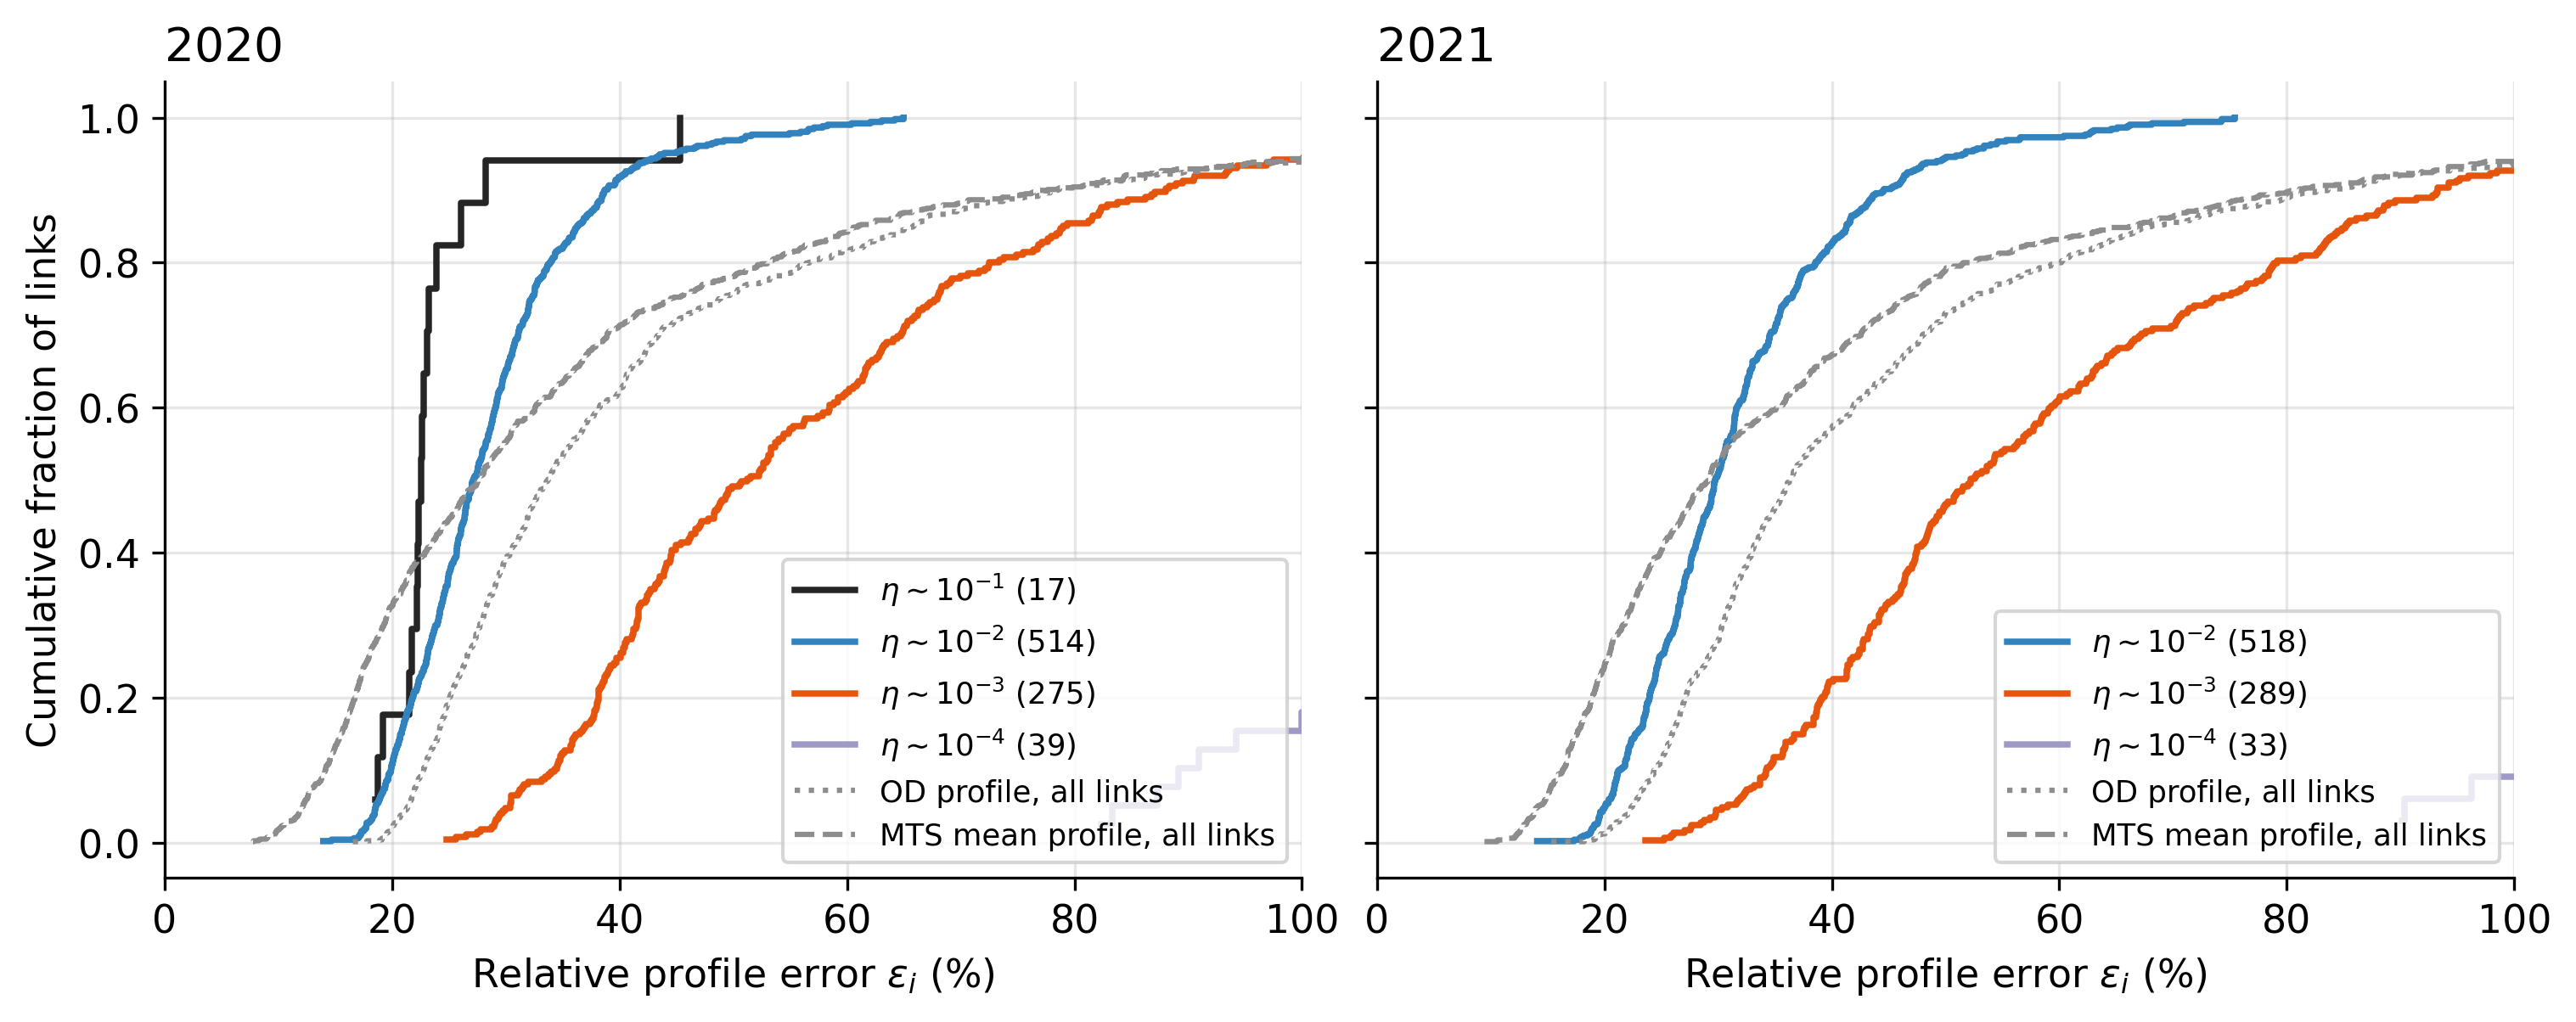
\includegraphics[width=\textwidth]{10_validation_cdf.png}
  \caption{\textbf{Profile error on all usable matched links.} Cumulative distribution of the relative error $\varepsilon_i$ (Eq.~\eqref{eq:relative_error}) by penetration class, with the number of links in parentheses, for 10--17 February 2020 (left) and 28 June--4 July 2021 (right). Grey curves: the same error when the OD demand profile (dotted) or the MTS mean profile (dashed) is used as prediction on every link.}
  \label{fig:validation_cdf}
\end{figure}

\subsection{Temporal subclusters and representative roads}

To show individual comparisons we take the 487 links of the upper class of a three-class $k$-means partition of $\log_{10}\eta_i$, which corresponds to $\eta_i\ge0.40\%$ in 2020. Their simulated profiles are normalized to hourly shares and clustered with Ward linkage and Euclidean distance \cite{ward1963,murtagh2014}; normalizing removes the volume of each road, so the clusters group links by the shape of their daily profile. Cutting the dendrogram into three clusters (Ward distance 0.15, Fig.~\ref{fig:subclusters}a) gives subclusters of 51, 78 and 358 links. Subcluster~1 has the sharpest morning peak (7.1\% of daily traffic at 07:00) and the fastest evening decline, subcluster~3 the flattest morning and the largest evening tail, and subcluster~2 lies in between (Supplementary Fig.~S2). The three subclusters are spread over the whole validation area (Fig.~\ref{fig:subclusters}b).

\begin{figure*}[htbp]
  \centering
  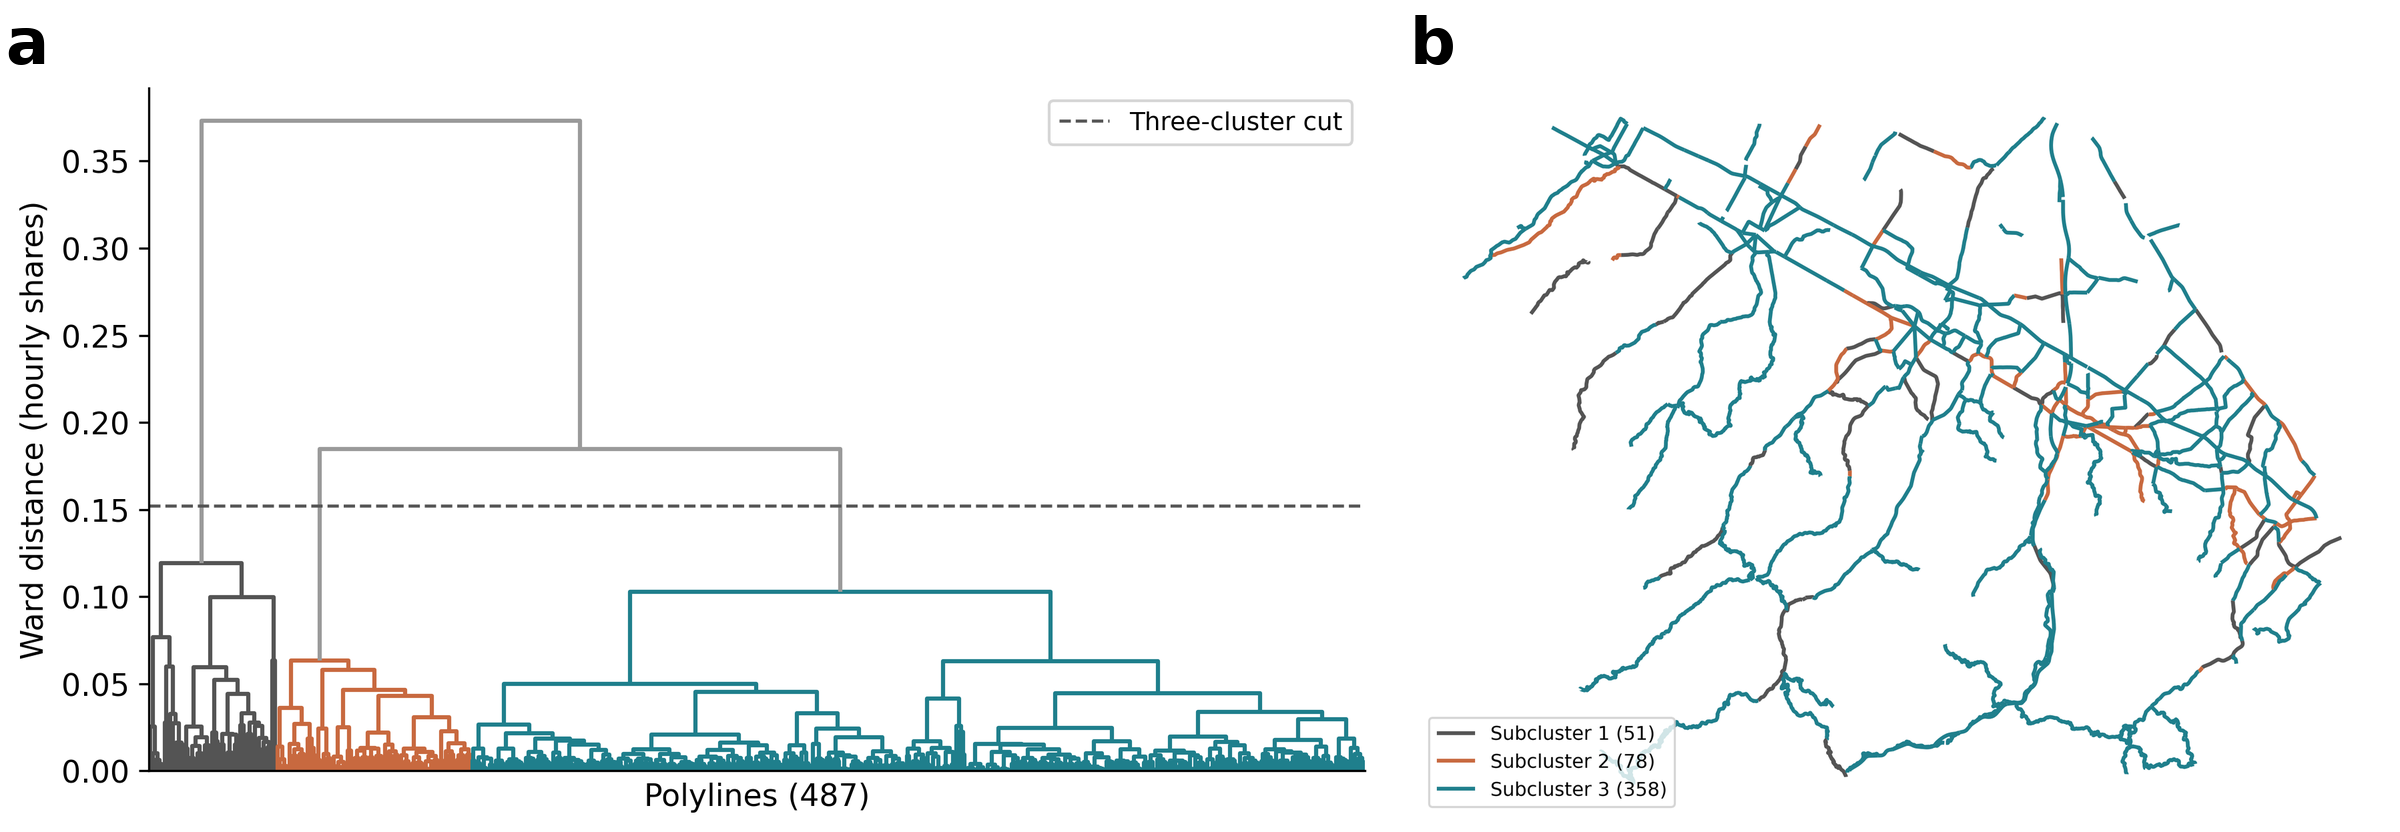
\includegraphics[width=\textwidth,height=.72\textheight,keepaspectratio]{fig5.png}
  \caption{\textbf{Subclusters of the high-penetration links in 2020.}
  \textbf{(a)} Ward dendrogram of the normalized hourly profiles of the 487 candidate links; the dashed line marks the three-cluster cut.
  \textbf{(b)} Location of the three subclusters, with the number of links in parentheses.}
  \label{fig:subclusters}
\end{figure*}

One link per subcluster is shown in Fig.~\ref{fig:representatives}. Polyline 104671 is kept because it lies close to the urban area of Forlimpopoli. The other two are the links of subclusters~2 and~3 with the lowest MAE among those at least 40~km from the other representatives: polylines 134419 and 64544. They are therefore best cases. Their MAE is 0.81 and 0.72~pp ($\varepsilon=19\%$ and 17\%), lower than on 95\% and 99\% of the usable links, while polyline 104671 has MAE $=1.22$~pp ($\varepsilon=29\%$), close to the median of the $\eta\sim10^{-2}$ class (Supplementary Section~S5). On all three roads the simulated morning rise precedes the GPS one by about an hour, which is the lead discussed above.

\begin{figure*}[htbp]
  \centering
  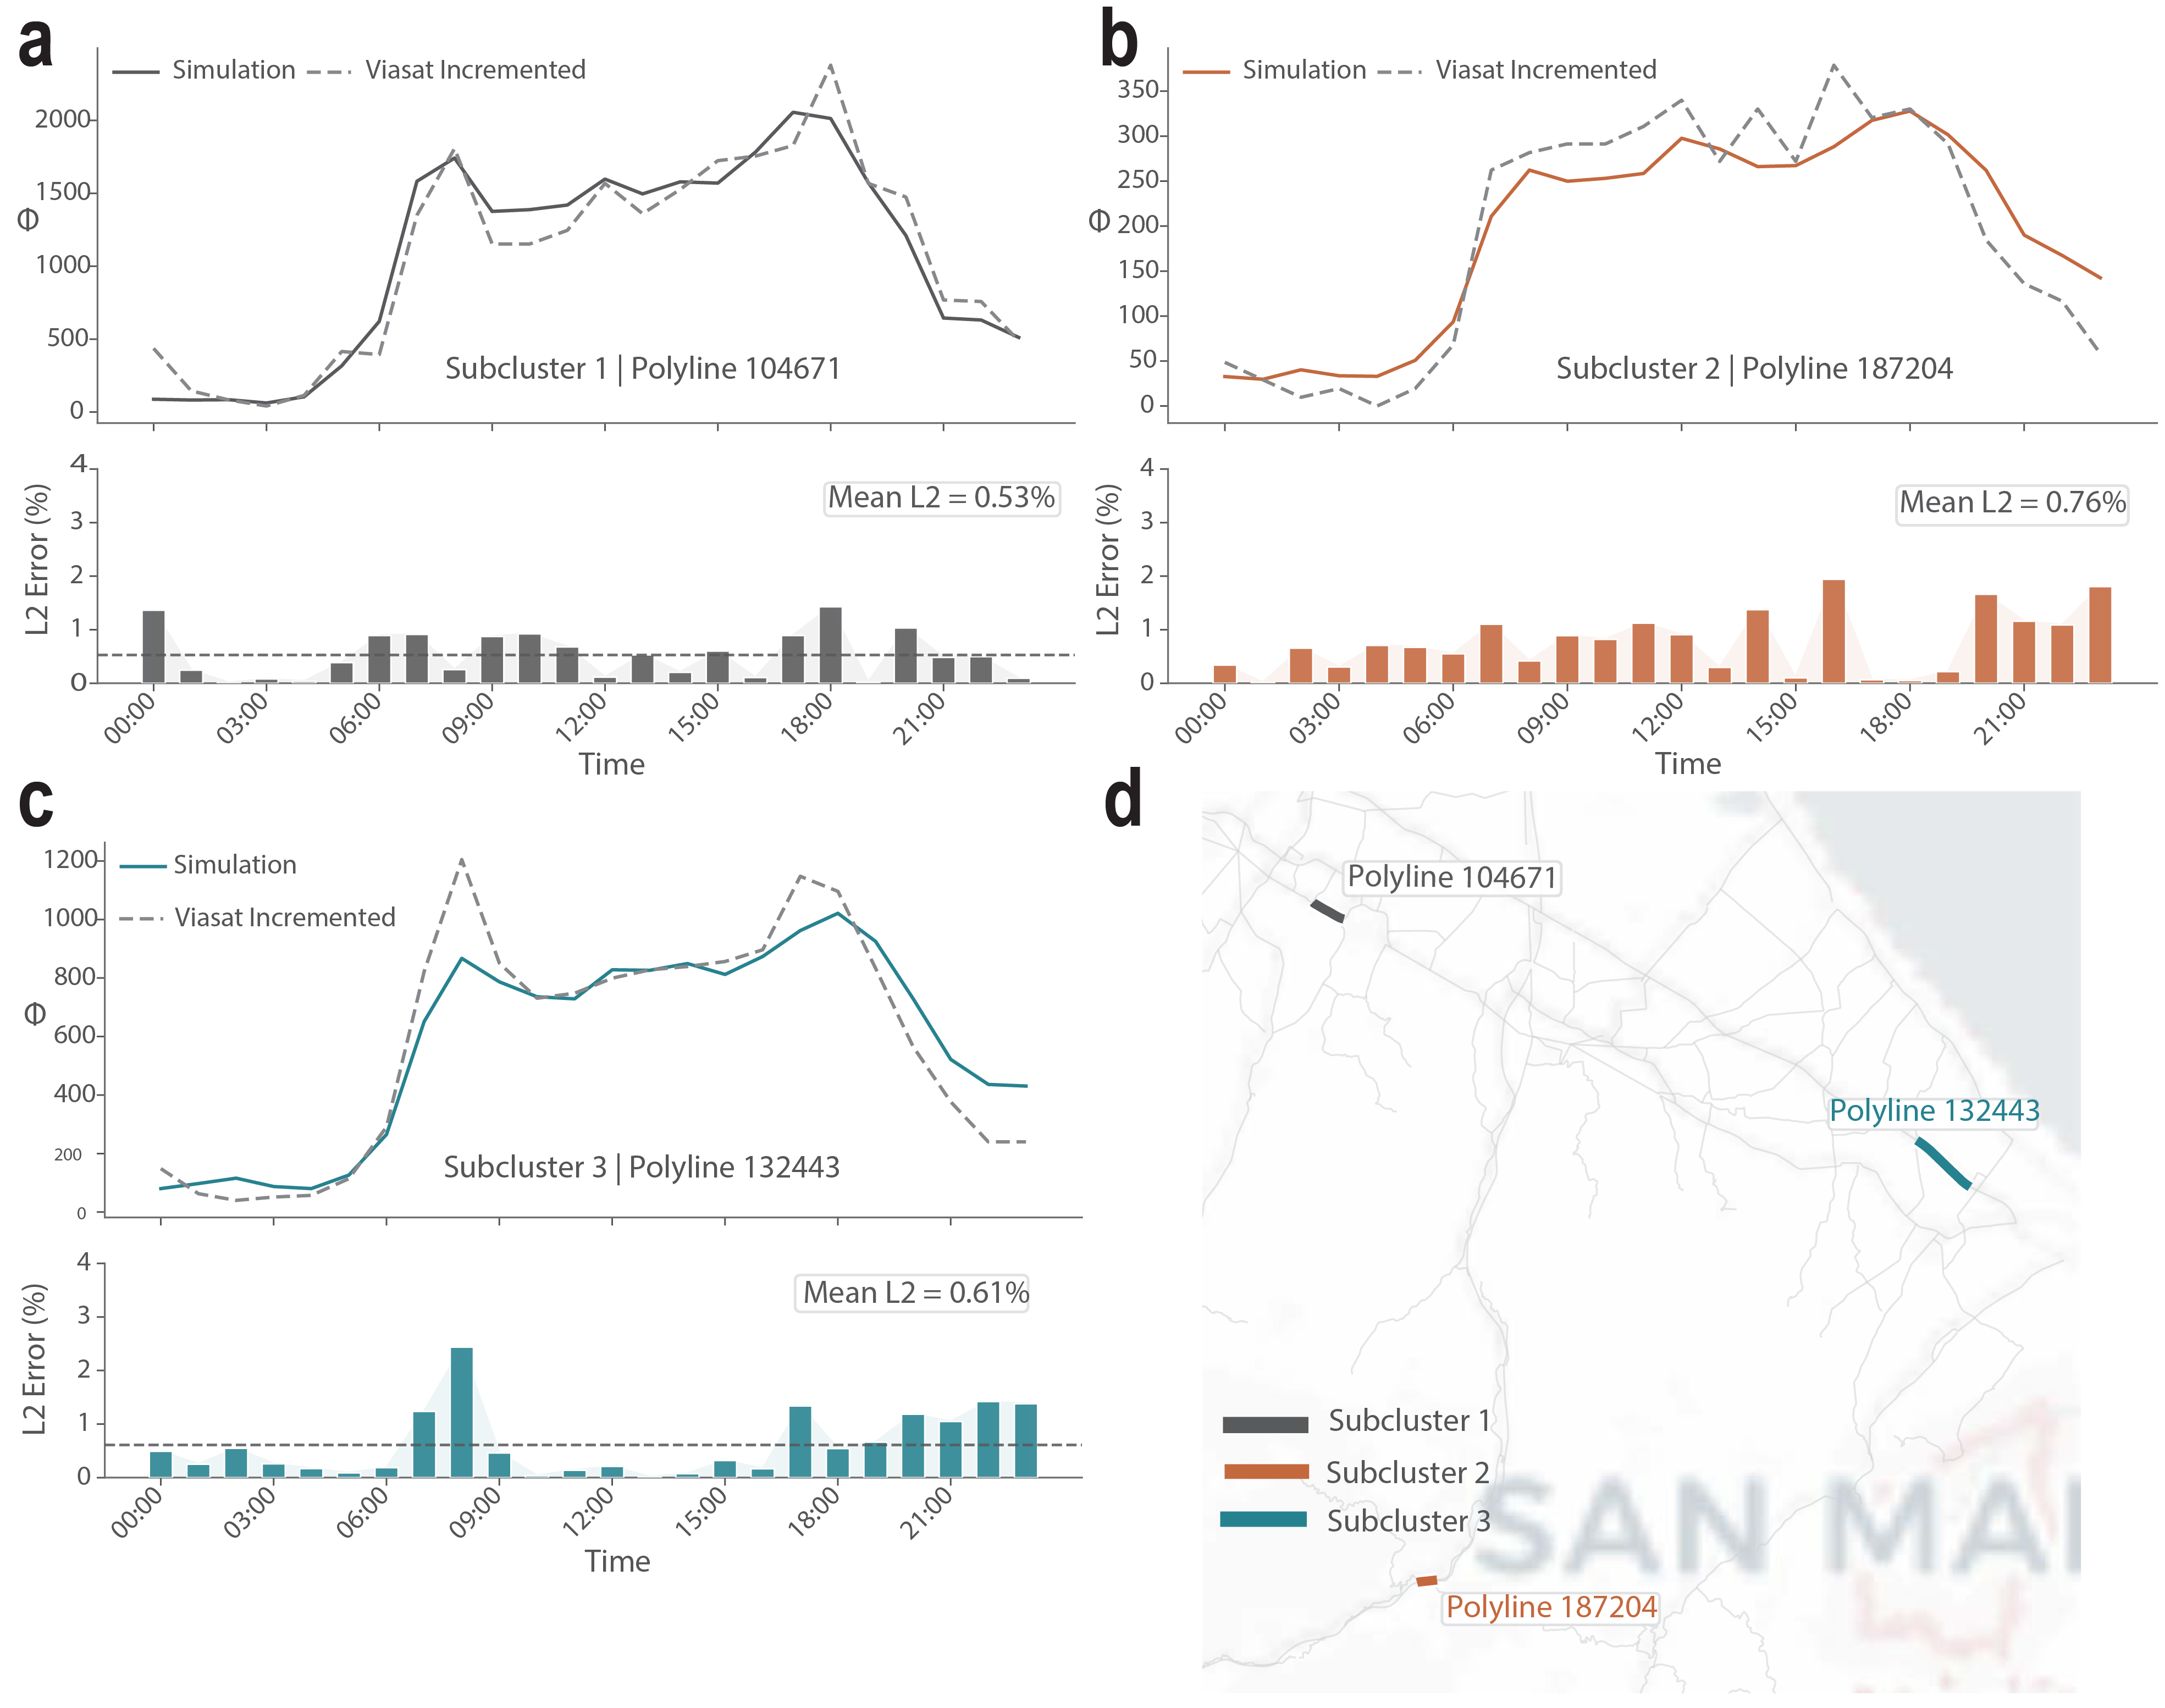
\includegraphics[width=\textwidth]{fig6.png}
  \caption{\textbf{Representative links, 10--17 February 2020.}
  \textbf{(a--c)} Mean simulated hourly flow and penetration-normalized Viasat profile (top) and hourly absolute share difference $|p_i(h)-q_i(h)|$ (bottom).
  \textbf{(a)} Subcluster 1, polyline 104671, MAE $=1.22$~pp.
  \textbf{(b)} Subcluster 2, polyline 134419, MAE $=0.81$~pp.
  \textbf{(c)} Subcluster 3, polyline 64544, MAE $=0.72$~pp.
  \textbf{(d)} Location of the three polylines on the road graph, coloured as in Fig.~\ref{fig:subclusters}.}
  \label{fig:representatives}
\end{figure*}

\subsection{Operational webserver}

The same chain runs as a webserver. An authenticated user selects a time interval in the browser; the backend builds the model configuration from the OD tables and the available coil data, runs \texttt{minimocas} in a separate process, applies the coil assimilation and stores the link-by-hour table with the run metadata (user, start time, runtime, status). Users can download the assimilated flows indexed by polyline and hour, plot the time series of selected links and map all polylines coloured by flow quantile. The dashboard also shows the MTS data (station maps, time series, rankings, clusters and anomaly diagnostics), so that counter quality and assimilation can be inspected in one place. Supplementary Section~S7 describes the components, the user workflow and the API.

\section{Methods}

\subsection{Data sources and preprocessing}\label{sec:data_preprocessing}

The road support is a routable regional graph derived from OpenStreetMap cartography. Road polylines are represented by local and cartographic identifiers, front and tail nodes, length and direction metadata. A preprocessed cartography file defines the node--polyline adjacency used both by the simulator and by the data-assimilation algorithm. The preprocessing follows standard graph-based principles for converting detailed cartography into a transport network that is simple enough to simulate while preserving the topological relations relevant to routing
\cite{osm,boeing2017,huynh2020,pung2022}.

Mobile-phone mobility is aggregated to municipality-level OD activity. The January 2020 records are separated into weekdays (Monday--Friday) and weekend days (Saturday--Sunday), with the public holidays of 1 and 6 January counted as weekdays, and into four generation classes: observed source--observed destination (\texttt{src-dest}), observed source--random destination (\texttt{src-rnd}), random source--observed destination (\texttt{rnd-dest}) and random source--random destination (\texttt{rnd-rnd}). These classes determine how origins and destinations are sampled when demand is injected into the simulation. The construction keeps the empirical OD component explicit and uses distance-aware random endpoints only for residual demand that cannot be assigned to two observed municipalities. The random-endpoint classes therefore act as a controlled residual mobility mechanism: they regularize sparse OD mass, preserve coverage of the regional graph and avoid forcing weakly observed flows into deterministic routes with spurious precision. This reflects the sensitivity of trip-distribution models to spatial support and missing observations
\cite{halas2014,lenormand2016,aste2015,little2019}.

MTS coil data are matched to road polylines through barrier metadata. A direction-pivot table maps registry directions to cartographic directions (\texttt{IN}/\texttt{OUT}). In the archived 2020 runs, short gaps in the observed coil series are filled by linear interpolation in time; for the 2021 runs no observed table in the project archive covers the simulated days, and the code falls back to weekday-specific seasonal average profiles. Viasat GPS data are independently map-matched to road polylines and are used only to validate the simulation framework; they are not used to assimilate or tune simulated flows. The meaning, scale and role of each data layer are summarized in Supplementary Section~S1.

\subsection{The \texttt{minimocas} traffic model}

\texttt{minimocas} is an agent-based traffic simulator in which each vehicle
is represented by an agent called "\texttt{pawn}". A pawn has a current polyline, a position along the polyline, a speed, a destination and a status. Simulation time advances with time step $\Delta t$; in the Emilia-Romagna configuration the code supports sub-hourly evolution and hourly camera dumps. During each time step, active pawns move along their current polyline. If they reach a node, the next polyline is chosen from the best-path matrix for the current destination, with an optional probability of missing the best path. The best-path matrix is computed on the weighted graph with a Dijkstra-style engine and respects no-turn constraints. The objective is not behavioural route-choice realism or dynamic congestion assignment. Shortest-path routing, the absence of adaptive rerouting and the simplified congestion rule are deliberate choices that favour stable reconstruction of aggregate directional flow fields from uncertain demand. The model is deliberately simpler than full microscopic platforms such as MATSim and SUMO
\cite{horni2016,lopez2018}, but it shares their agent-based representation
of trips and network loading.

Sources inject new pawns according to time-varying creation rates. The daily creation-rate vector is indexed by simulation time, allowing the mobile-phone hourly demand profile to modulate the number of generated trips. Depending on the generation class, the model can use observed origins and destinations, draw one missing endpoint conditionally, or draw both endpoints from the regional node set. The selected OD pair is converted into an initial directed polyline and a destination node; the pawn then follows the network until the trip is completed or killed by model rules.

The simulator records two forms of traffic output. Barrier counters count crossings at coil-like virtual barriers. Unique polyline output records, for each dump interval and each direction, the number of distinct pawn identifiers present on a polyline. This second output is the link-level quantity used in the reconstructed flow maps and in the subsequent data-assimilation step.

The model also updates link velocities from simulated density. For each polyline $i$, density is the number of pawns on the link divided by its length. The code imposes a critical-density rule: above the critical density the link speed is set to a critical speed; below it, the nominal polyline speed is linearly reduced with density. The link flow used internally is the product of density and updated speed. This places the implementation within the broader family of traffic-flow and car-following models that link microscopic motion to macroscopic density, speed and flow
\cite{nagel1992,bando1995,helbing1998,jiang2001,bham2004,helbing2001,brackstone1999,newell2002,treiber2013}.
Supplementary Section~S2 provides the run inventory and source-class counts, while Supplementary Section~S3 describes the model-state variables.

\subsection{Coil-based data assimilation}

The data-assimilation procedure implemented in the framework adjusts the
simulated unique-link matrix using MTS coil residuals. Let $u_i(h)$ denote
the simulated unique count on the polyline associated with coil $i$,
$b_i(h)$ the corresponding synthetic barrier count, and $c_i(h)$ the
observed coil count after direction mapping and temporal harmonization. The
code first estimates the relation between barrier and unique counts,
\begin{equation}
  r_i(h) = \frac{b_i(h)}{\max(u_i(h),1)} ,
  \label{eq:barrier_unique_ratio}
\end{equation}
and computes a relative residual in barrier space,
\begin{equation}
  \Delta_i(h) =
  \frac{c_i(h) r_i(h) - b_i(h)}
       {\max(b_i(h),1)} .
  \label{eq:coil_residual}
\end{equation}
The residual is turned into an additive increment on the directed coil link,
\begin{equation}
  \delta_i(h) = u_i(h)\,\Delta_i(h), \qquad
  \tilde u_i(h) = u_i(h) + \delta_i(h) ,
  \label{eq:assimilation_increment}
\end{equation}
which is applied only when $\tilde u_i(h)>0$. Whenever $u_i(h)\ge 1$ and $b_i(h)\ge 1$, Eqs.~\eqref{eq:barrier_unique_ratio}--\eqref{eq:assimilation_increment} give $\tilde u_i(h)=c_i(h)$: on the coil link the assimilated count equals the observation. Negative counts produced by the propagation are clipped to zero. Fixed counters therefore constrain the simulated field where they exist, and the simulation supplies the spatial structure used to pass this information to nearby links \cite{herrera2010,seo2017}; this is a local correction, not a calibration of the whole network.

The increment is propagated recursively through adjacent directed links with turning weights taken from the simulated unique counts. For an incoming link $(n_1,n_2)$ and an admissible outgoing link $(n_2,n)$,
\begin{equation}
  \delta_{(n_2,n)}(h) = w_{(n_1,n_2)\to n}(h)\,\delta_{(n_1,n_2)}(h), \qquad
  w_{(n_1,n_2)\to n}(h) = \frac{u_{(n_2,n)}(h)}{\sum_{m} u_{(n_2,m)}(h)} ,
  \label{eq:propagation}
\end{equation}
where the sum runs over the admissible outgoing links; when their simulated counts are missing the split is uniform. A backward recursion with the analogous upstream weights distributes the same increment to the incoming links. In the runs analysed here the recursion stops when the propagated increment falls below one vehicle, after three links, when the next node gives access to another coil polyline, or when a forbidden turn or a closed polyline would be crossed. The assimilated table keeps the directional unique-polyline format of the simulator output. Areas far from reliable counters receive no correction and remain as uncertain as the raw simulation. Supplementary Section~S4 lists the stopping rules and the differences between the archived implementation and the one now running in the webserver.

\subsection{Accident exposure and hazard-weighted traffic}

The accident data are the hourly tables of road accidents with injuries in Emilia-Romagna for 2022, 2023 and 2024, averaged over the three years; they pool all days of the week. Exposure comes from twelve weekday runs, one in each month of 2023, and eleven Sunday runs of the same year, all driven by the OD matrices of Section~\ref{sec:data_preprocessing}.

Let $\phi_i(h)$ be the simulated flow on link $i$ during hour $h$. Hourly exposure is obtained by summing simulated traffic over the road network,
\begin{equation}
  E(h) =
  \frac{\sum_i \phi_i(h)}
       {\sum_{h'}\sum_i \phi_i(h')} ,
  \label{eq:exposure_share}
\end{equation}
so that $E(h)$ is a daily share. Accident counts are normalized in the same way,
\begin{equation}
  A(h) =
  \frac{a(h)}
       {\sum_{h'} a(h')} ,
  \label{eq:accident_share}
\end{equation}
where $a(h)$ is the mean number of accidents in hour $h$, and $R(h)$ follows from Eq.~\eqref{eq:hourly_risk}. Weekday and weekend exposure give two versions of $R(h)$; the link indicators below use the weekday one.

The hazard-weighted exposure of link $i$ is
\begin{equation}
  H_i = \sum_h \phi_i(h) R(h) .
  \label{eq:hazard_weighted_exposure}
\end{equation}
and the weekday--weekend contrast is
\begin{equation}
  D_i =
  \frac{H_i^{\mathrm{weekday}} - H_i^{\mathrm{weekend}}}
       {H_i^{\mathrm{weekday}} + H_i^{\mathrm{weekend}}} ,
  \label{eq:weekday_weekend_hazard_difference}
\end{equation}
evaluated where the denominator is positive. The risk centrality
\begin{equation}
  C_i = \frac{H_i}{\sum_j H_j} ,
  \label{eq:risk_centrality}
\end{equation}
is the share of the total hazard-weighted exposure carried by link $i$, and the rank difference
\begin{equation}
  S_i = \operatorname{rank}(H_i) - \operatorname{rank}(E_i),
  \label{eq:hazard_anomaly}
\end{equation}
compares the percentile rank of $H_i$ with that of the total simulated exposure $E_i=\sum_h \phi_i(h)$ among the links with $E_i>0$. Figure~\ref{fig:spatial_risk}e highlights the links in the top 5\% of $S_i$.

\subsection{GPS validation and clustering}

Validation uses Viasat only after matching GPS roads with simulated polylines. The GPS data are not used to generate demand, assimilate coil residuals, tune the simulation or select model parameters. They provide an external check of the temporal profiles produced by the reconstruction framework. For every matched road, the link-specific penetration coefficient in Eq.~\eqref{eq:penetration} rescales the GPS series so that total volume on that road is aligned before profile comparison. Because this scaling uses each road separately, it tests the temporal profile on that physical link rather than a region-wide sum or a universal market-penetration factor. The MAE of hourly shares in Eq.~\eqref{eq:profile_error} is used as the hourly validation diagnostic because absolute probe counts are not total traffic counts: Viasat observes a partial fleet, and its penetration varies across links. Normalization isolates whether the simulated and observed profiles rise, peak and decline at comparable hours, which is the validation target for the reconstructed temporal field. This is a conservative use of probe data: the GPS traces validate shape and timing after penetration adjustment, but they are not treated as complete traffic counts and are not merged back into the calibration or data-assimilation stages \cite{seo2015,seo2017,bellisardi2025}.

The examples of Fig.~\ref{fig:representatives} are chosen as described in the Results: Ward clustering of the normalized simulated profiles of the high-penetration links, one link per subcluster, with polyline 104671 fixed and the other two selected by lowest MAE under a 40~km separation constraint. Supplementary Section~S5 lists the selection steps and the metrics of the selected links.

\section{Discussion}

The main methodological contribution is the construction of an operational reconstruction chain in which heterogeneous mobility sensors keep explicit semantic roles. Mobile-phone records define the regional demand signal; the road graph and simulator perform the network assignment; coils provide local data assimilation where direct counts exist; and Viasat is reserved for independent temporal-profile validation of the simulation framework. Each observational layer preserves its original measurement meaning, and the workflow explicitly separates demand generation, routing, data assimilation and validation. This separation is important because each layer has a different sampling mechanism and a different spatial support. It also follows a central lesson of urban analytics: large mobility data sets are powerful when their observation process is kept visible, not when they are treated as complete observations
\cite{zheng2014,kitchin2014,kitchin2016,kandt2021}.

The validation results show that the simulation framework can produce reconstructed daily profiles consistent with held-out, penetration-normalized GPS profiles on illustrative roads from three temporal subclusters. At the same time, the penetration maps and supplementary validation tables make clear that validation strength is not uniform over the entire cartography. The workflow is therefore best interpreted as a transparent data-fusion and validation pipeline, not as proof that every low-penetration road is reconstructed with the same accuracy. This validation focuses on temporal-profile consistency after penetration normalization, rather than on absolute fleet-size estimation. The latter would require additional assumptions and data sources, such as fleet composition, vehicle-kilometres travelled, fuel sales or regional population. The current strategy is more conservative: it tests whether the temporal dynamics produced by the reconstruction framework are consistent with an independent probe-vehicle sample after link-specific normalization, but it does not estimate a universal GPS market share or claim absolute calibration of all links.

The practical value of the workflow is that it produces a road-level traffic representation from data sources that are normally used separately. This output can be used to identify corridors with high reconstructed flows, compare weekday and weekend demand scenarios, inspect the temporal profile of specific roads, support local traffic-management decisions and provide an exposure layer for downstream analyses such as emissions, noise, road-safety screening or infrastructure stress. Because the reconstructed quantity is indexed by road polyline and time, it can also be aggregated after the fact to municipalities, provinces, corridors or user-defined areas without re-running the model. Planning tools and regional digital twins need this kind of intermediate layer \cite{batty2013,peldon2024}.

The accident analysis uses the reconstructed field as an exposure denominator. With aggregate tables, normalization changes the reading of the hourly counts: the hours around midnight have few accidents but an even smaller simulated exposure, and therefore the highest $R(h)$, while the busy day hours fall below one. The exponent $\alpha=0.72$ (0.58--0.88) means that across hours the accident share grows less than proportionally with exposure. Speed regime, visibility, road environment and reporting can all contribute \cite{elvik2005,aarts2006}, and the present data cannot separate them. Because $R(h)$ is regional, the link maps rank roads by the hourly composition of their simulated traffic; geolocated accident records would be needed to test whether the highlighted links are more dangerous.

The webserver implementation is important because it operationalizes the validated reconstruction workflow without changing its scientific assumptions. It turns the offline chain into a repeatable service: a user can choose a time window, launch the simulation, monitor progress, download data-assimilated flows and visualize the result on the road graph. This makes the workflow suitable for reproducible scenario analysis, operational reporting and communication with stakeholders who need interpretable traffic fields as maps and tables rather than source code. The dashboard also keeps the MTS monitoring layer close to the simulation layer, allowing counter data quality, anomalies and data-assimilation behaviour to be inspected in the same environment. The detailed service architecture is summarized in Supplementary Section~S7.

The main limitation of the present implementation is the seasonal support of the OD matrix. The demand layer used here is based on winter mobility observations, and therefore represents a specific seasonal configuration of regional mobility. Access to multiple OD matrices, ideally derived from different data sources and covering different seasons, would allow the same framework to reproduce seasonal changes in mobility demand more explicitly and to test how robust the reconstructed link-flow field is under different demand regimes.

A second limitation is methodological and operational. The simulator is intentionally simplified to keep regional runs compatible with webserver deployment and interactive stakeholder use. It does not implement a full dynamic congestion mechanism or adaptive traffic assignment; instead, it uses shortest-path network loading together with a free-flow/threshold velocity representation. This choice is coherent with the main target of the study, which is the reconstruction of aggregate directional flows on a large extra-urban road network rather than the detailed modelling of urban congestion waves. Within this setting, the coil-based data-assimilation step is the mechanism that anchors simulated flows to local observations while preserving feasible runtimes for repeated operational analyses.

Future work should therefore focus on extending the demand basis and testing the model under richer seasonal and multi-source OD scenarios. On the operational side, the webserver could be extended with explicit scenario controls, seasonal demand selection, user-defined regions of interest and automatic reporting of the OD and sensor layers used in each run.

\section{Conclusions}

This work presents a regional-scale workflow for reconstructing road traffic flows by combining mobile-phone activity, fixed traffic counters, OpenStreetMap cartography and GPS telemetry. The contribution is not a new routing algorithm, but an interpretable multi-layer reconstruction framework in which demand generation, network loading, local data assimilation and independent validation remain explicitly separated. The proposed chain integrates heterogeneous mobility observations into a coherent time-dependent traffic field at the road-link scale over a large regional network.

Held-out Viasat telemetry validates the simulation framework by showing strong consistency between reconstructed and GPS-derived hourly profiles on representative roads from different temporal mobility regimes after link-specific penetration normalization. This should be interpreted as a validation of reconstructed temporal dynamics rather than as a claim of complete absolute calibration across the entire network. The results nevertheless show that large-scale mobility patterns can be reconstructed with sufficient temporal and spatial coherence to support downstream operational analyses.

The same field can serve as an exposure layer for aggregate accident statistics. Normalized by simulated exposure, the hourly accident share of 2022--2024 gives a relative risk that peaks around midnight and stays below one after 19:00, and across hours the accident share scales as $E^{0.72}$. The link maps derived from this regional profile rank roads by the hourly composition of their traffic, and can indicate where geolocated accident data or local counts should be collected first.

Beyond scientific analysis, the workflow was designed with stakeholder-oriented applications in mind. The dashboard implementation supports simulation management, monitoring, visualization and export of reconstructed flows, enabling regional analysts to inspect mobility scenarios without directly interacting with the modelling pipeline. Potential applications include congestion screening, infrastructure stress assessment, environmental-impact analysis, exposure-based safety prioritization and digital-twin support for regional mobility management.

Future developments should incorporate uncertainty quantification, systematic sensitivity analyses for the data-assimilation procedure and broader validation campaigns across additional territories and temporal conditions. Further extensions could integrate weather conditions, road characteristics and near-real-time mobility observations to support predictive hazard assessment and adaptive traffic-management strategies.


\section*{Supplementary Material}

Supplementary Material provides tabular documentation of the data layers, simulation runs, \texttt{minimocas} state variables, data-assimilation rules, validation metrics, accident descriptors and webserver architecture referenced throughout the main text. Supplementary Fig.~S1 reports additional descriptive statistics on accident totals, road environment and seasonal shares, and Supplementary Section~S8 summarizes reproducibility notes for the reported counts, thresholds and operational workflow.

\section*{Availability of data and materials}

Processed figure inputs and the code required to regenerate the analyses are available in the project repository. Public traffic-counter data from the Emilia-Romagna Region are available through the MTS online mobility platform at \url{https://mobilita.regione.emilia-romagna.it/servizi/flussi-online}. Road-accident statistics are publicly available from ISTAT at \url{https://www.istat.it/tag/incidenti-stradali/}. Mobile-phone and Viasat GPS datasets used in this study are proprietary and cannot be publicly distributed.


\section*{Competing interests}

The authors declare that they have no competing interests.

\section*{Funding}

FB acknowledges financial support from the Italian National Operational Programme on Research and Innovation 2014--2020 (CCI 2014IT16M2OP005), funded through FSE REACT-EU resources under Action IV.4 'Doctorates and research contracts on innovation topics' and Action IV.5 'Doctorates on Green topics'.

\section*{Authors' contributions}

FB conceived part of the original study design, developed the reconstruction workflow, performed the analyses and prepared the first manuscript draft. CM and AF contributed to the development of the modelling framework. AB contributed to the study design, interpretation of the modelling results and manuscript revision. All authors read and approved the final manuscript.

\section*{Acknowledgements}

The authors gratefully acknowledge Telecom for providing the datasets and technical support that made this work possible. We also thank the Mobility and Viability Section of the Emilia-Romagna Region for their collaboration and support. In particular, we thank Stefano Grandi, Claudio Domenichini and Elena Grossi for their valuable assistance and insights throughout the development of the project.


\bibliographystyle{unsrtnat}
\bibliography{references}


\end{document}
